\section{Electromagnetic Models}

In this section, we explore how the vector fitting and interconnection methods can be used for characterizing electromagnetic models of superconducting circuits. To obtain the multiport impedance parameters needed for our characterization methods, we use Ansys HFSS \cite{ansys_hfss} for the full-wave FEM electromagnetic simulations and Qiskit Metal \cite{Qiskit_Metal} for some of the device modeling. Also, when working with some of the simulation results we have used the Python package scikit-rf \cite{scikit_rf}.

\subsection{Brick Building Approach}

Simulating a full electromagnetic model of a multi-qubit superconducting circuit can be prohibitively expensive if trying to obtain the impedance parameter over a broad frequency range. To tackle this, we propose a method where circuit designs can be broken up into smaller and simpler ``bricks". Then, these pieces can be interconnected to obtain a model of a larger device. Since the number of ports and resonant modes for each of these bricks will be much smaller than for the full model, applying the fitting methods of Section \ref{section:vector_fitting} is possible. If we have the rational impedances of multiple bricks, we can then use the method of Section \ref{section:rational_impedance_interconnection} to obtain the rational impedance function of the larger interconnected model. From this rational impedance function, we can easily construct a circuit Hamiltonian.

Splitting up your circuit does not come without compromise. For example, capacitive coupling between qubits in different bricks will not be taken into account accurately. However, since we obtain the full Hamiltonian of the system, any potential cross-brick coupling that is not taken into account can be added in afterwards. For this, we would need to estimate the long range capacitive coupling of the components in the circuit, which can be done using formulas for planar electrodes \cite{planar_capacitance} or potentially with simpler capacitance only simulations.

To see an example of the brick building method in action, we look at how it can be applied to the model in Fig.\ \ref{fig:cap_res_cap_full}. The circuit in Fig.\ \ref{fig:cap_res_cap_full} is a two port network which contains a half-wave coplanar waveguide (CPW) resonator that is capacitively coupled to the two ports. In this simulation and the ones that follow, the models will contain perfectly conducting sheets on top of a silicon substrate. Sometimes, wirebonds are also included over meandered CPWs. Wave ports are used for the ports located at the boundary of the model. We will compare the simulation results of this model to the split model as shown in Fig.\ \ref{fig:cap_res_cap_split}.

\begin{figure}[!h]
    \centering
    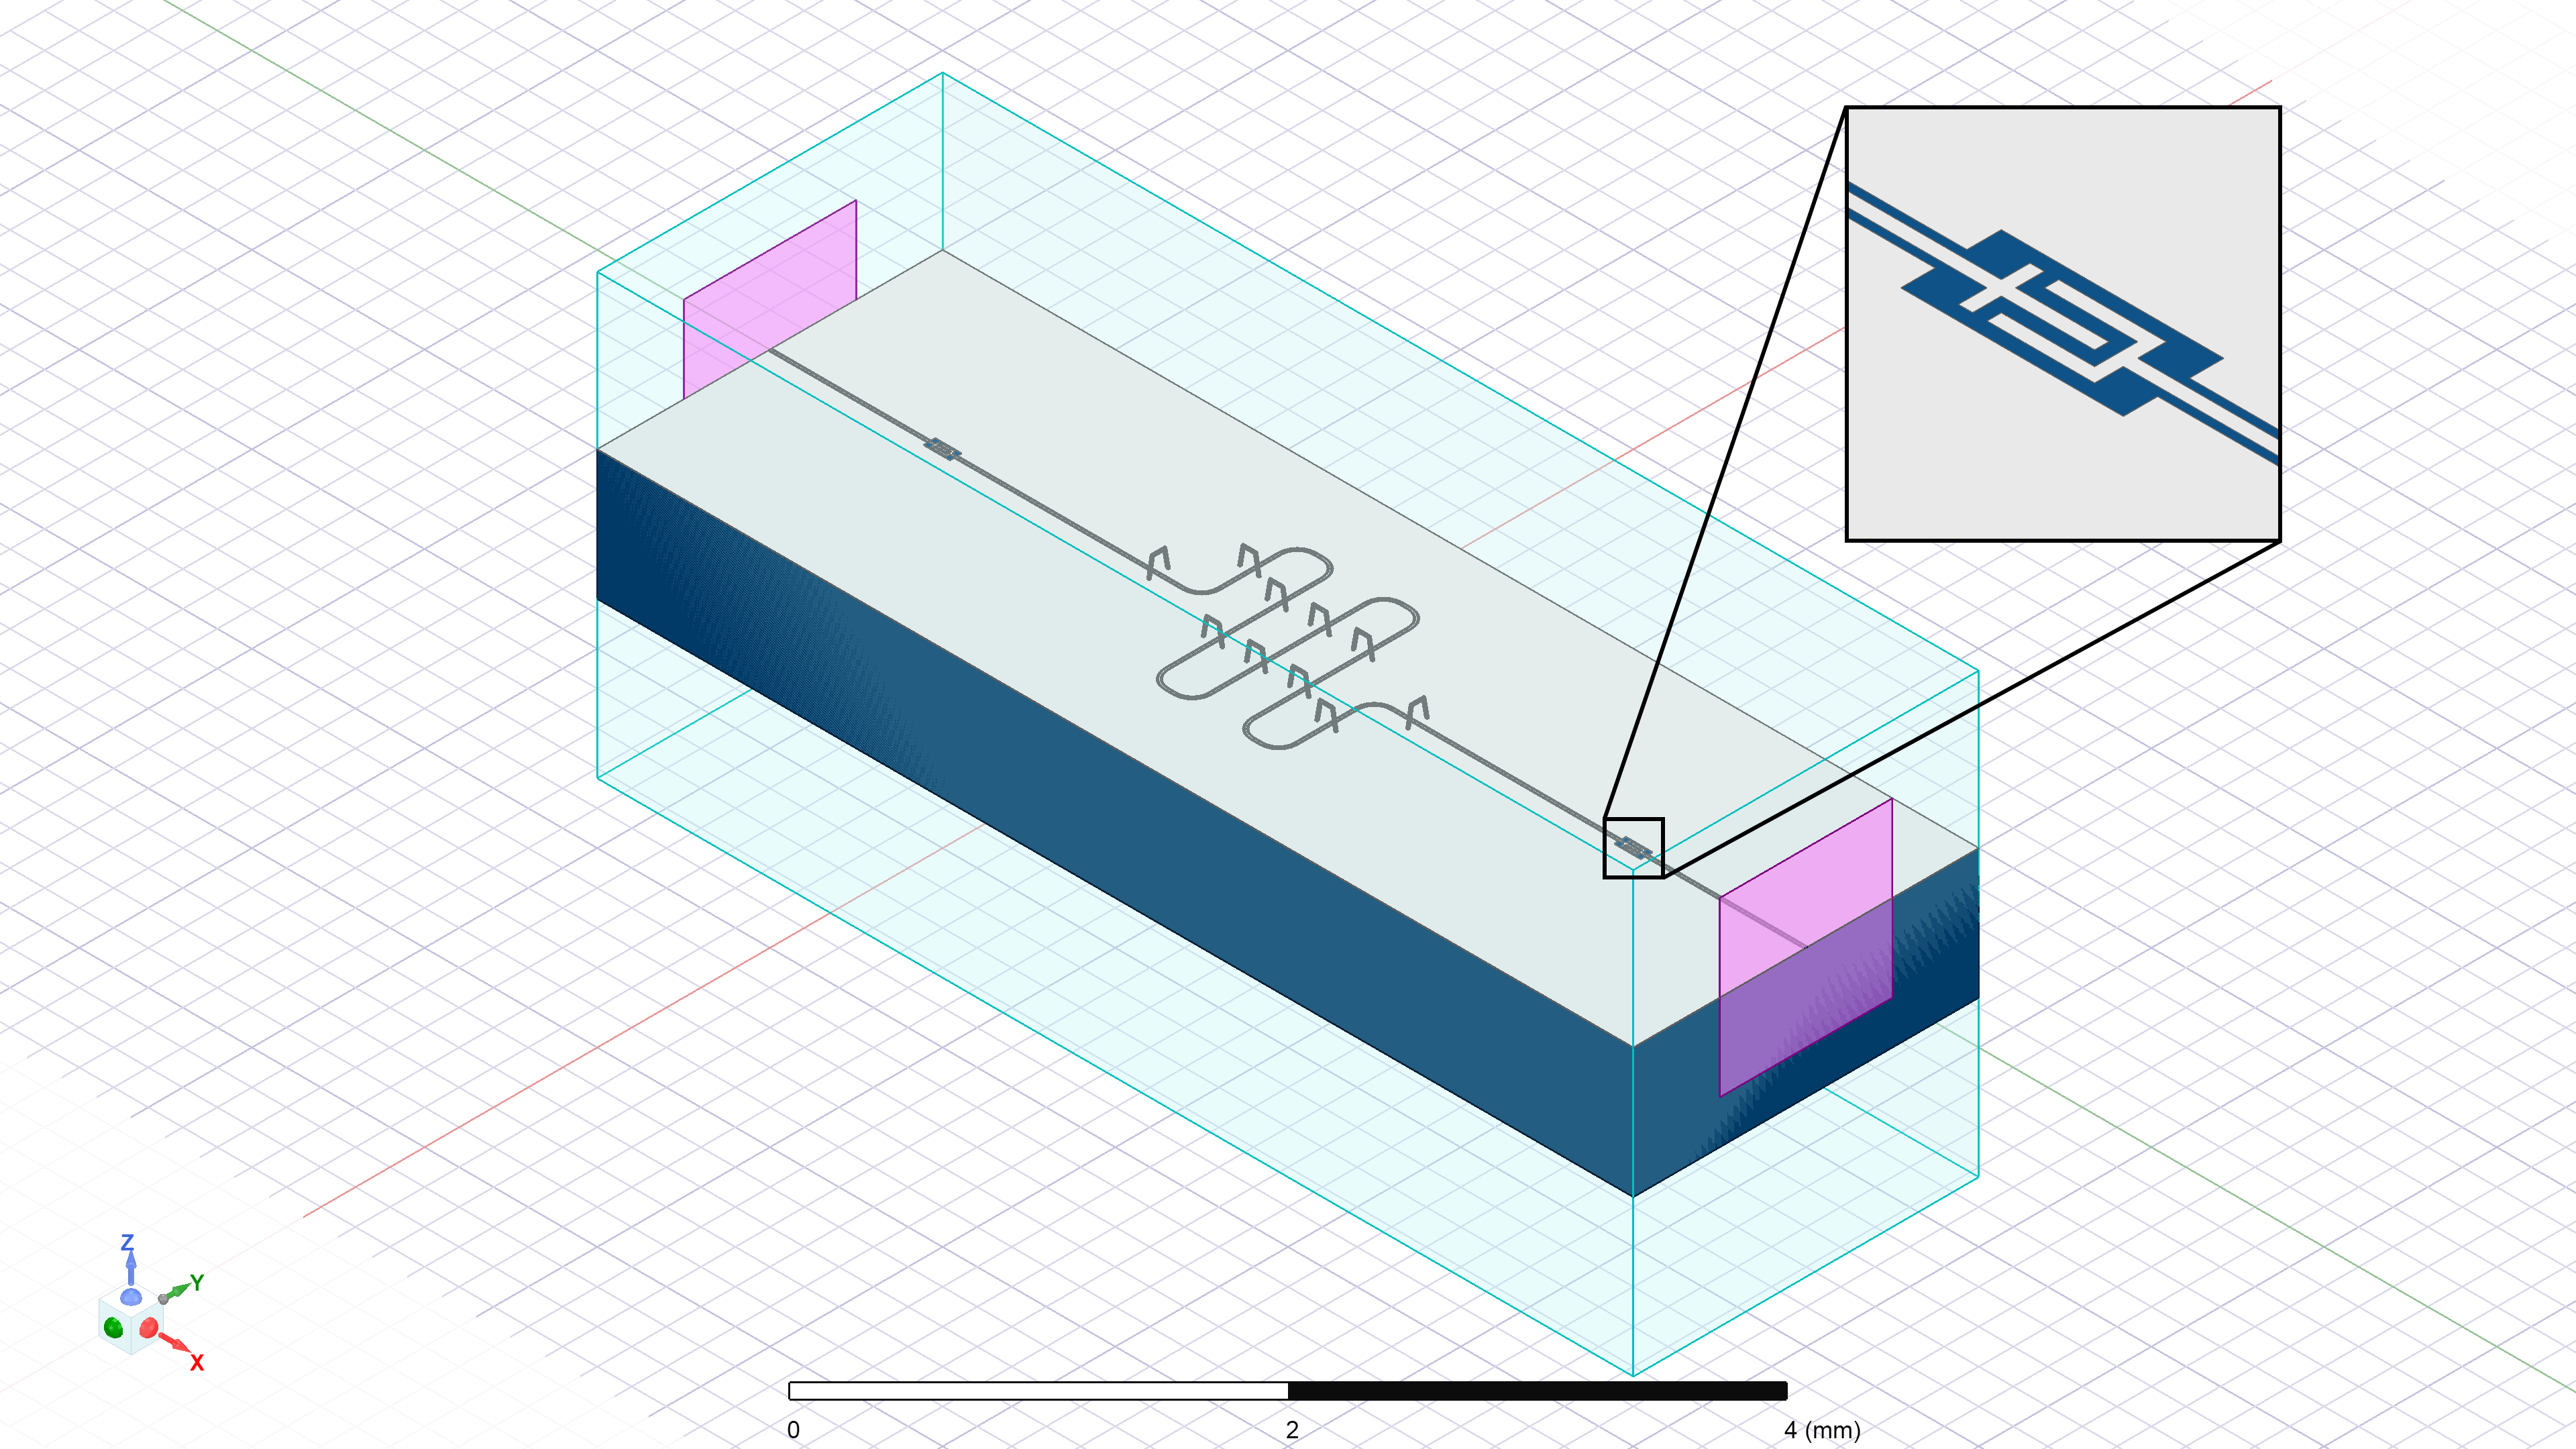
\includegraphics[width=\textwidth]{figures/cap_res_cap_full.png}
    \caption{Two port circuit containing an 8 mm half-wave CPW resonator that is capacitively coupled to the two external ports.}
    \label{fig:cap_res_cap_full}
\end{figure}

\begin{figure}[!h]
    \centering
    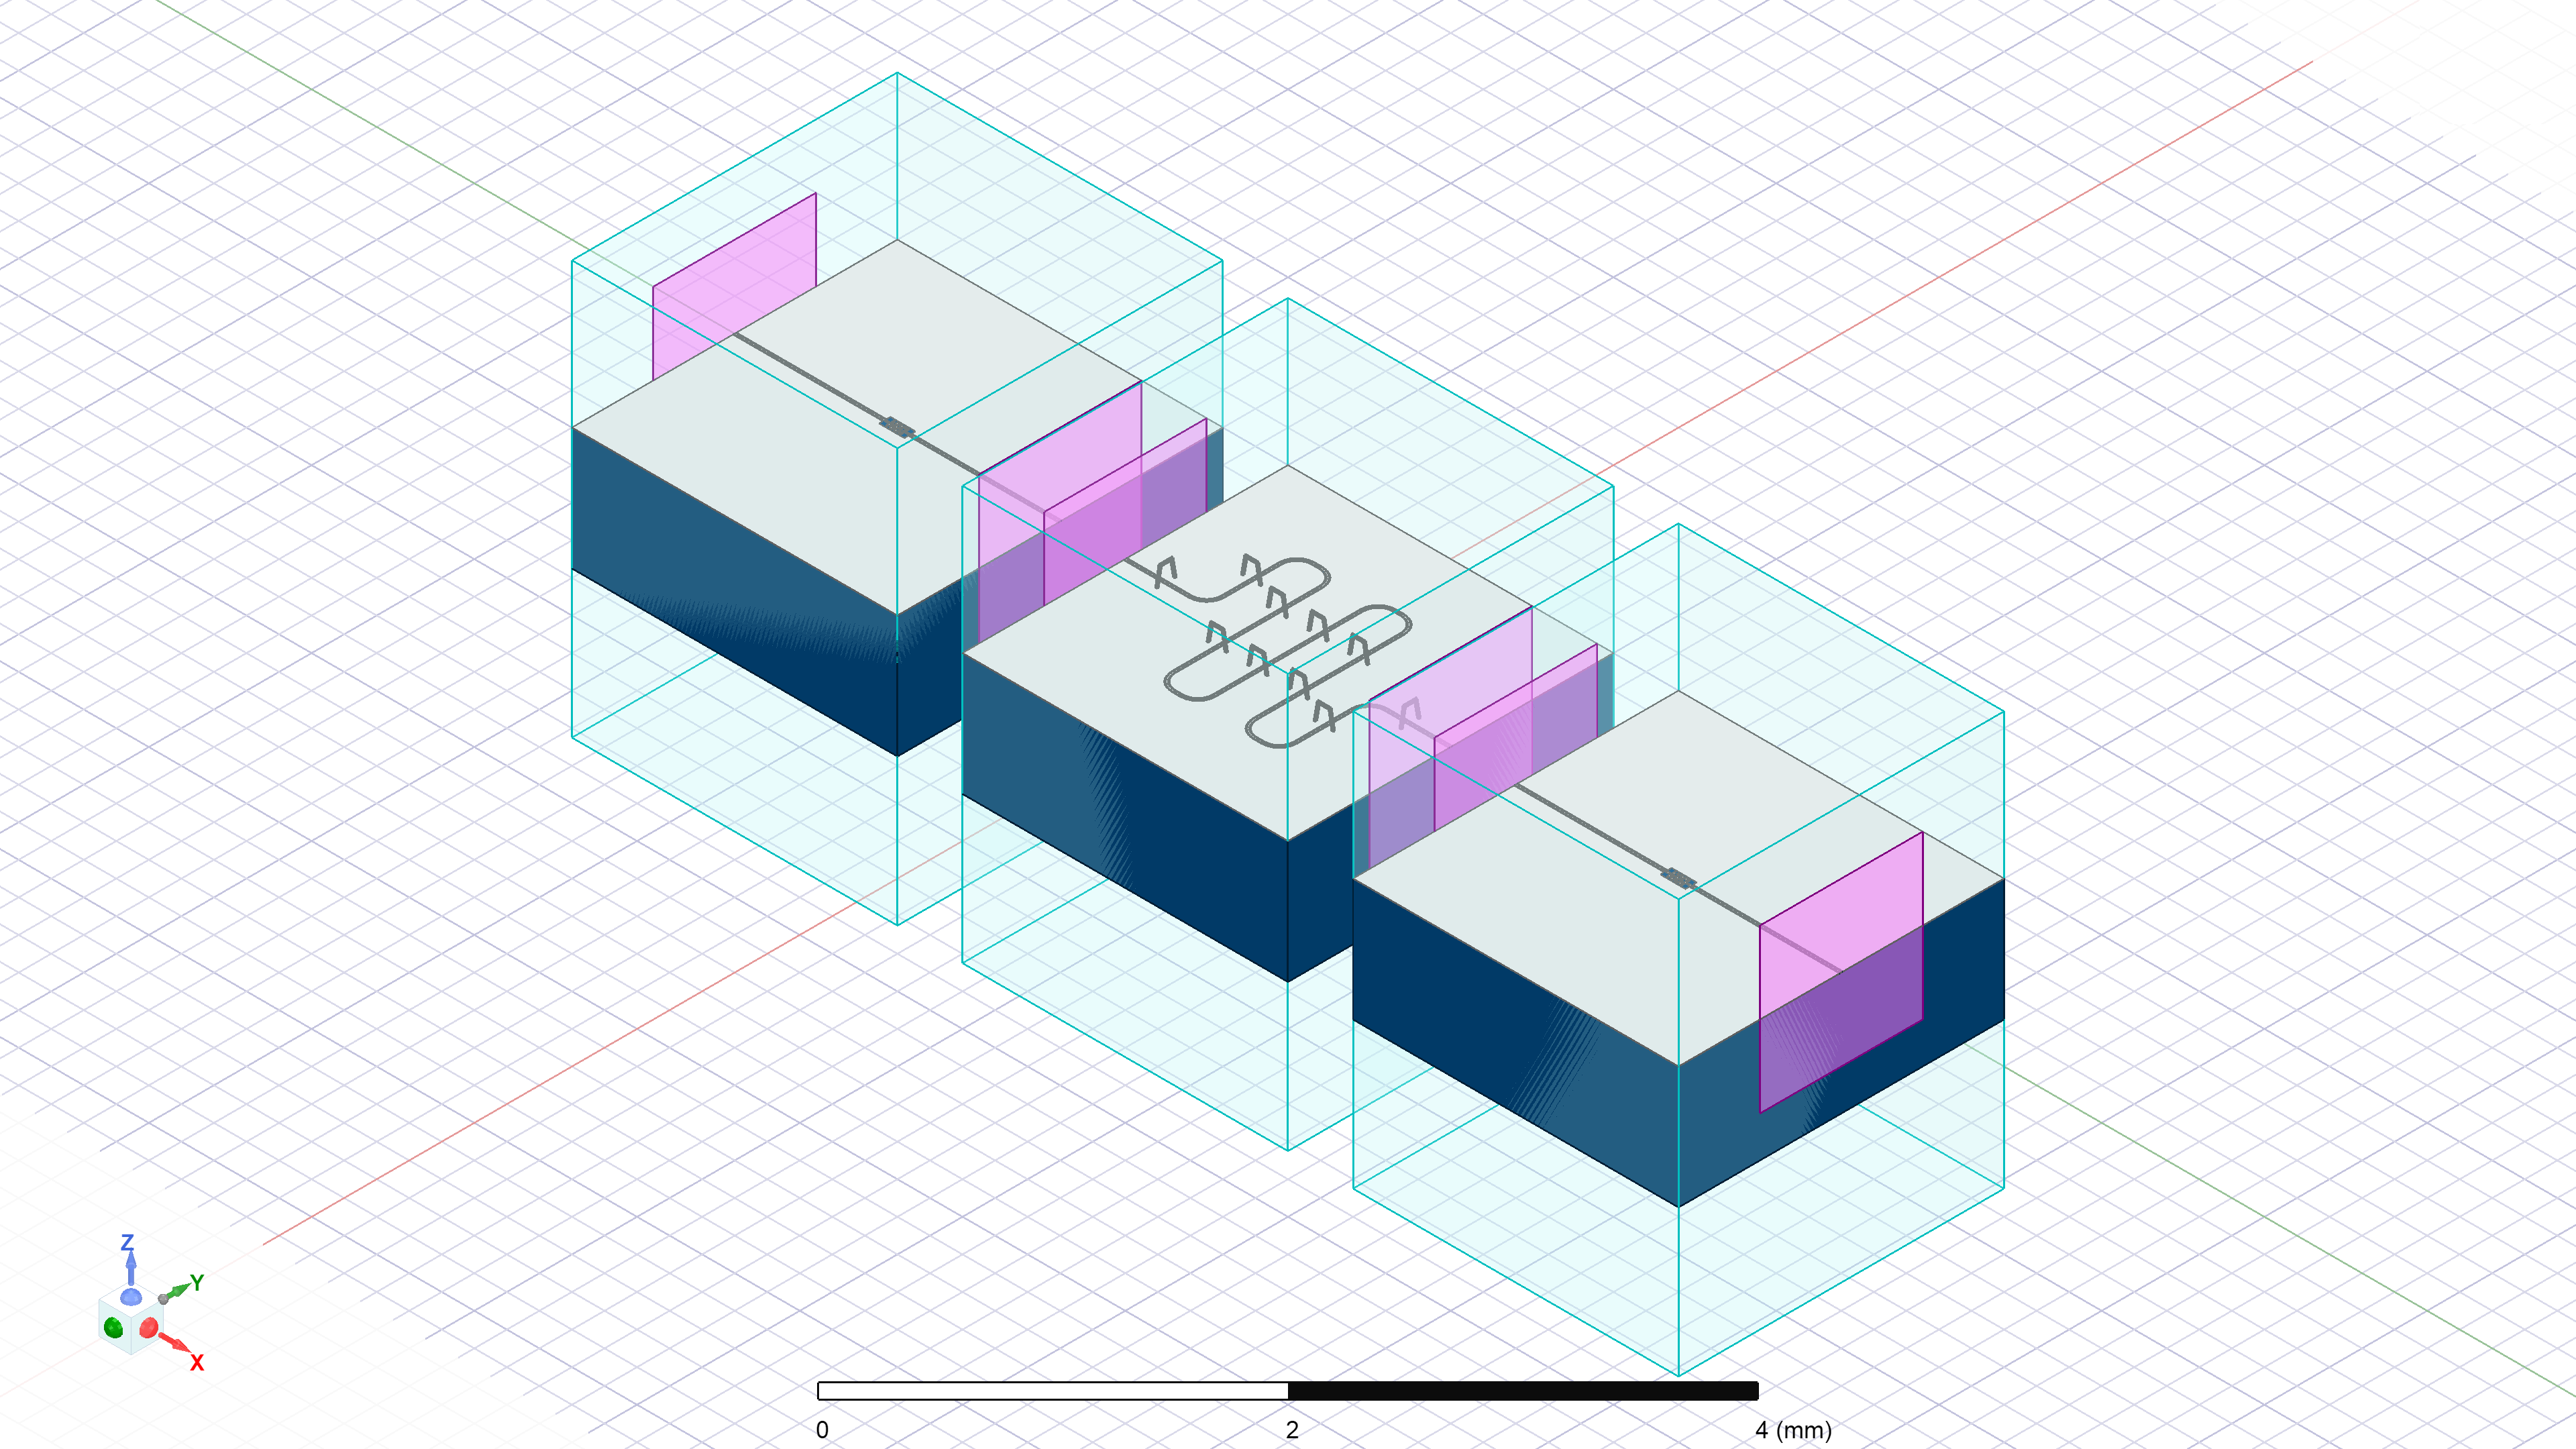
\includegraphics[width=\textwidth]{figures/cap_res_cap_split.png}
    \caption{Split version of the model in Fig.\ \ref{fig:cap_res_cap_full}. The left and right bricks are identical and only contain the finger capacitor coupled to the two ends with CPWs. The center brick only contains a 6 mm CPW.}
    \label{fig:cap_res_cap_split}
\end{figure}

For all of our simulations we will use the interpolating sweep options in HFSS, where the software chooses at what frequencies to solve the model, and then interpolates the solution with its own fitting methods. The model is repeatedly solved and fitted until the difference in S-parameters between runs is under a specified percentage. We have chosen an error tolerance of 0.5\% for these examples. Alternatively, we could pick these frequency points ourselves and apply the fitting methods directly. We are also using the adaptive fitting methods within HFSS to obtain a mesh that has a convergence at the high end of the our chosen frequency range (20.5 GHz). The mesh for the model in Fig.\ \ref{fig:cap_res_cap_full} is shown in Fig.\ \ref{fig:cap_res_cap_mesh}.

We then apply the fitting process from Section \ref{section:vector_fitting} to the simulations of the bricks in Fig.\ \ref{fig:cap_res_cap_split}. The results of the fitting are shown in Fig.\ \ref{fig:cap_res_fit}. Then, using the interconnection method of Section \ref{section:rational_impedance_interconnection}, we can stitch bricks together to obtain a final rational impedance function. To show the difference between the full model and the brick model, we compare the $S_{12}$ parameters in Fig.\ \ref{fig:full_vs_brick}. In this comparison, we see that primary differences are in the resonance frequencies of the full model and the brick model. We estimate that the resonance frequency of the fundamental mode in the brick model is approximately 15 MHz higher ($+0.2$\%) compared to the full model. We also confirm that this is not due to the fitting by comparing the interconnected model before and after the fit and finding a negligible difference. This suggests that the modeling of these bricks can be improved. One potential cause of the difference is the meshes for the full and split models. To improve on this, we could potentially decrease the error tolerance for the adaptive meshing process which in this case is at 1\%. We could also make the adaptive meshing process sample results from more frequency points. Another potential problem with the split model could be the dimensions of the wave ports. These points in addition to other components such as the interpolating sweeps and even comparison with other simulation software should be explored further in any implementations of this splitting method.

\begin{figure}[!t]
    \centering
    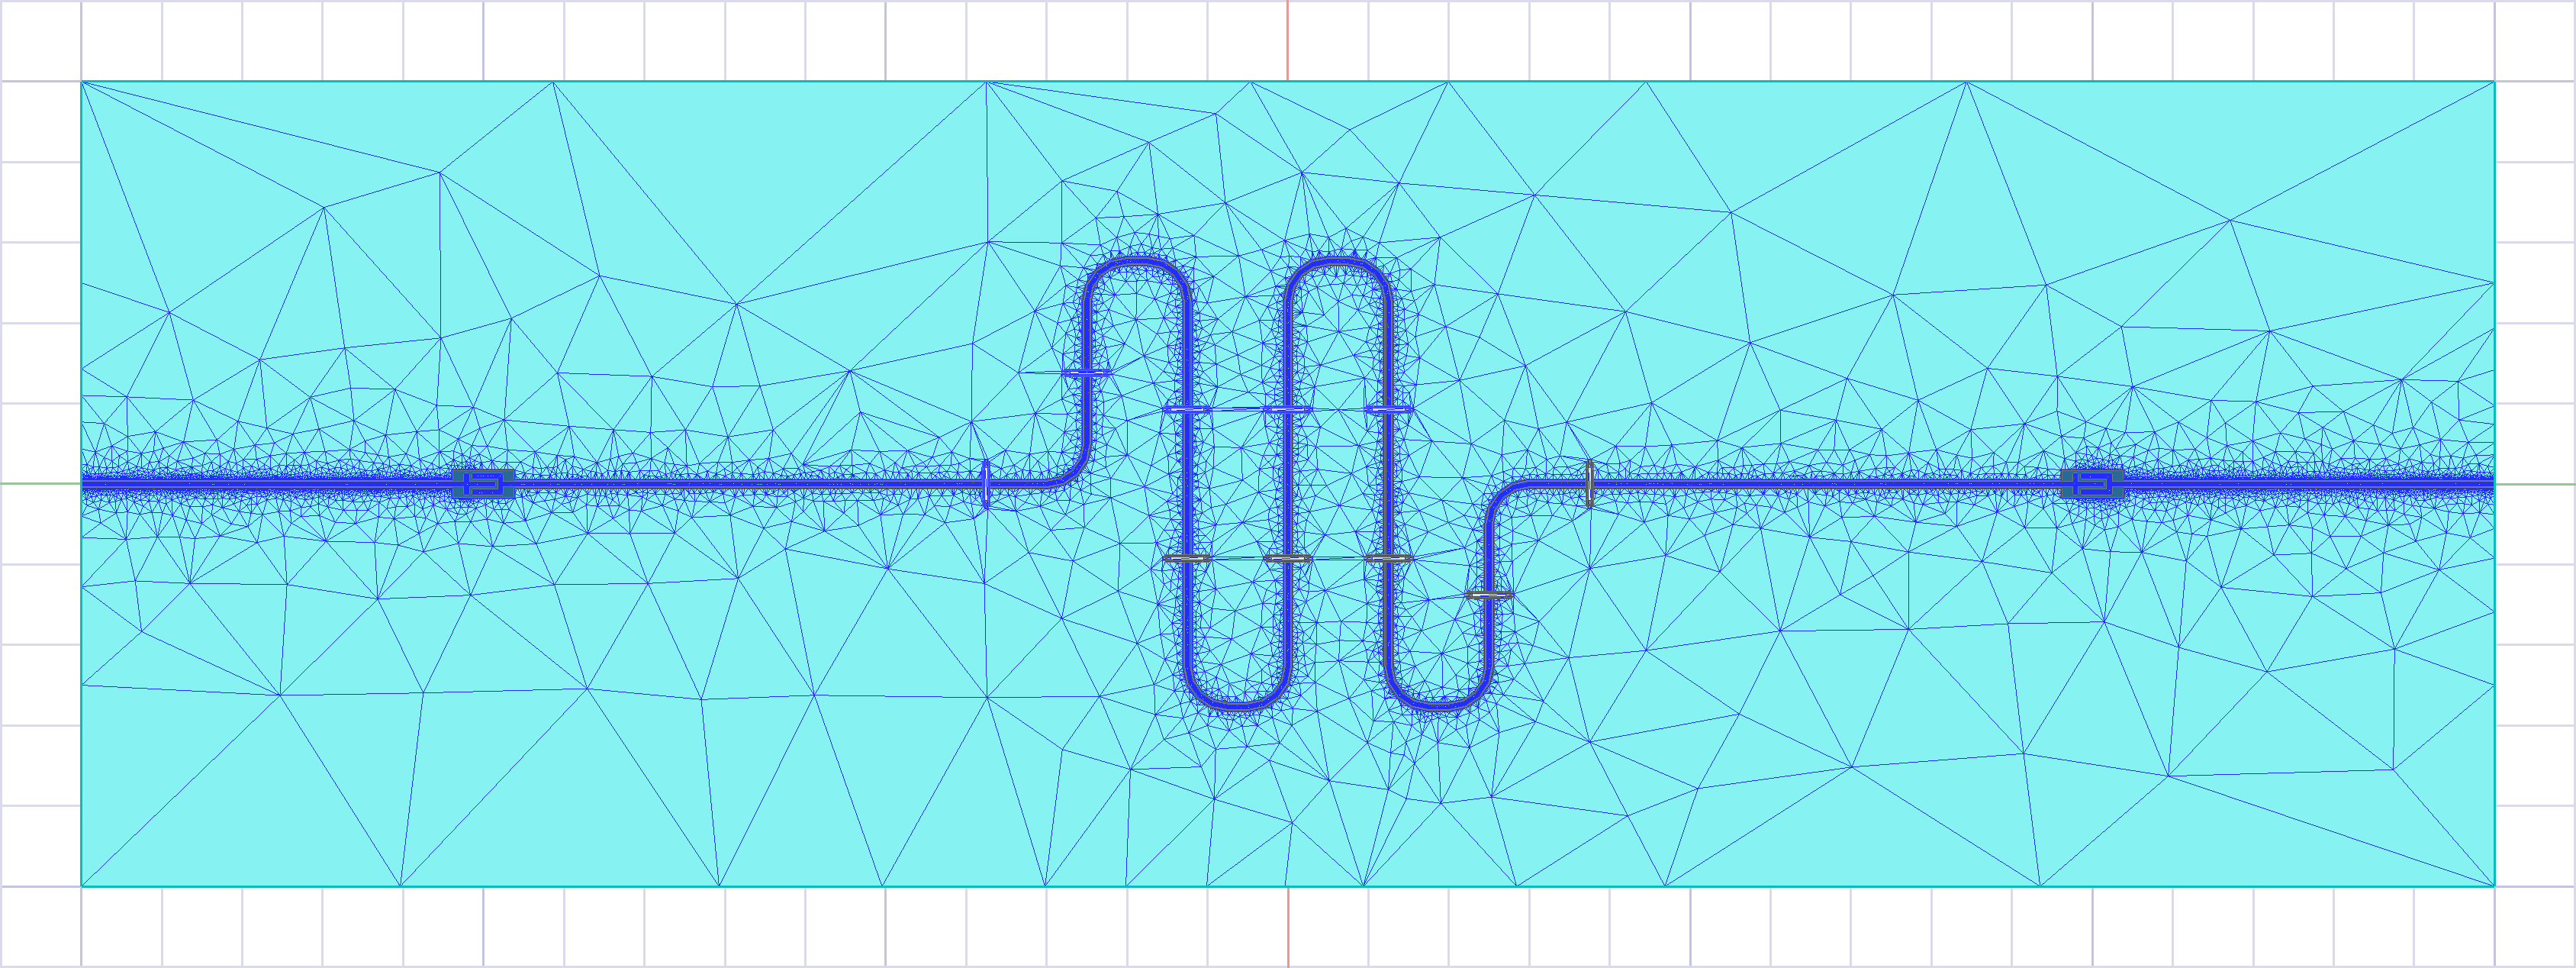
\includegraphics[width=\textwidth]{figures/cap_res_cap_mesh.png}
    \caption{Mesh used for the simulation of the model in Fig.\ \ref{fig:cap_res_cap_full}.}
    \label{fig:cap_res_cap_mesh}
\end{figure}

\begin{figure}[!t]
    \centering
    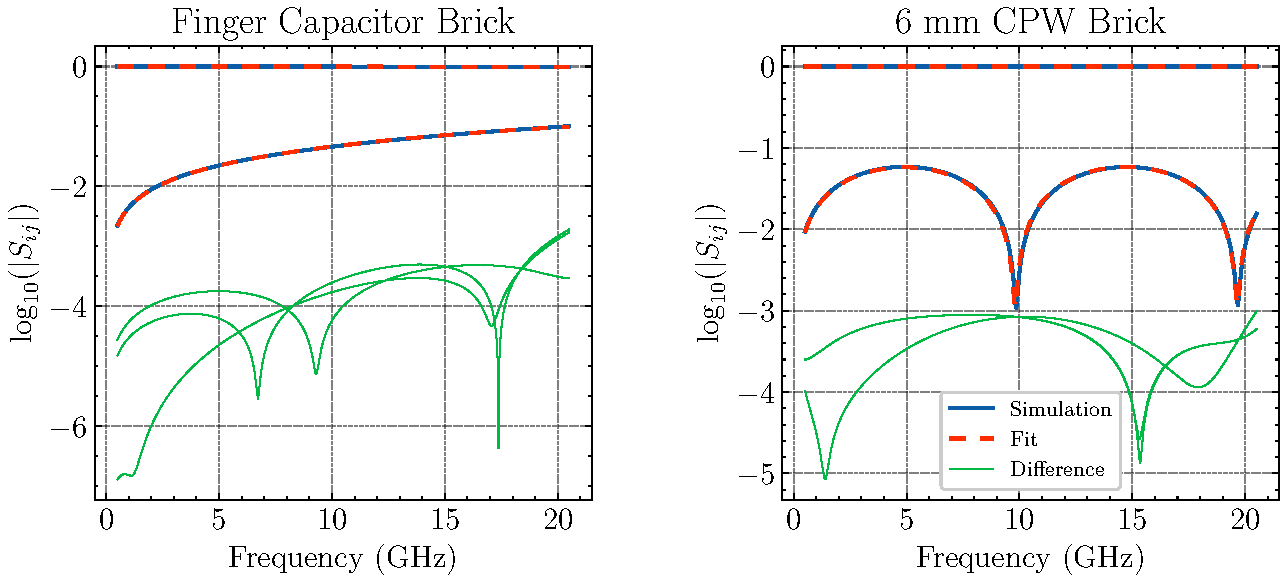
\includegraphics[width=\textwidth]{figures/cap_res_fit.pdf}
    \caption{Fitting results for the capacitor and CPW bricks shown in Fig.\ \ref{fig:cap_res_cap_split}. After converting the fitted rational impedance function to S-parameters, it is compared to the S-parameters from the simulation. All the S-parameters and differences are plotted on the same plot.}
    \label{fig:cap_res_fit}
\end{figure}

\begin{figure}[!h]
    \centering
    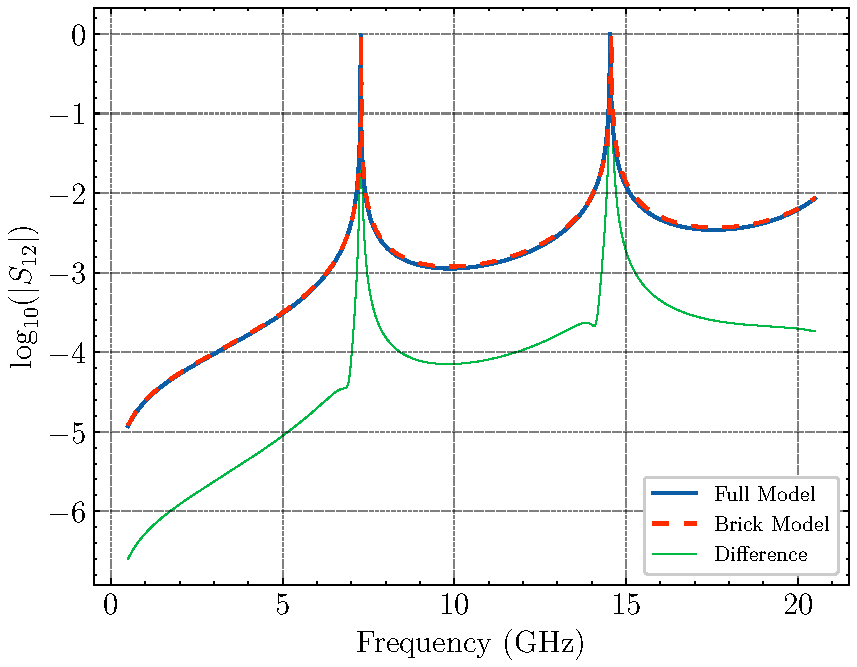
\includegraphics[width=0.6\textwidth]{figures/full_vs_brick.pdf}
    \caption{Difference between the $S_{12}$ parameter from the simulation of the full model in Fig.\ \ref{fig:cap_res_cap_full} and the interconnected brick model in Fig.\ \ref{fig:cap_res_cap_split}.}
    \label{fig:full_vs_brick}
\end{figure}

\begin{figure}[!h]
    \centering
    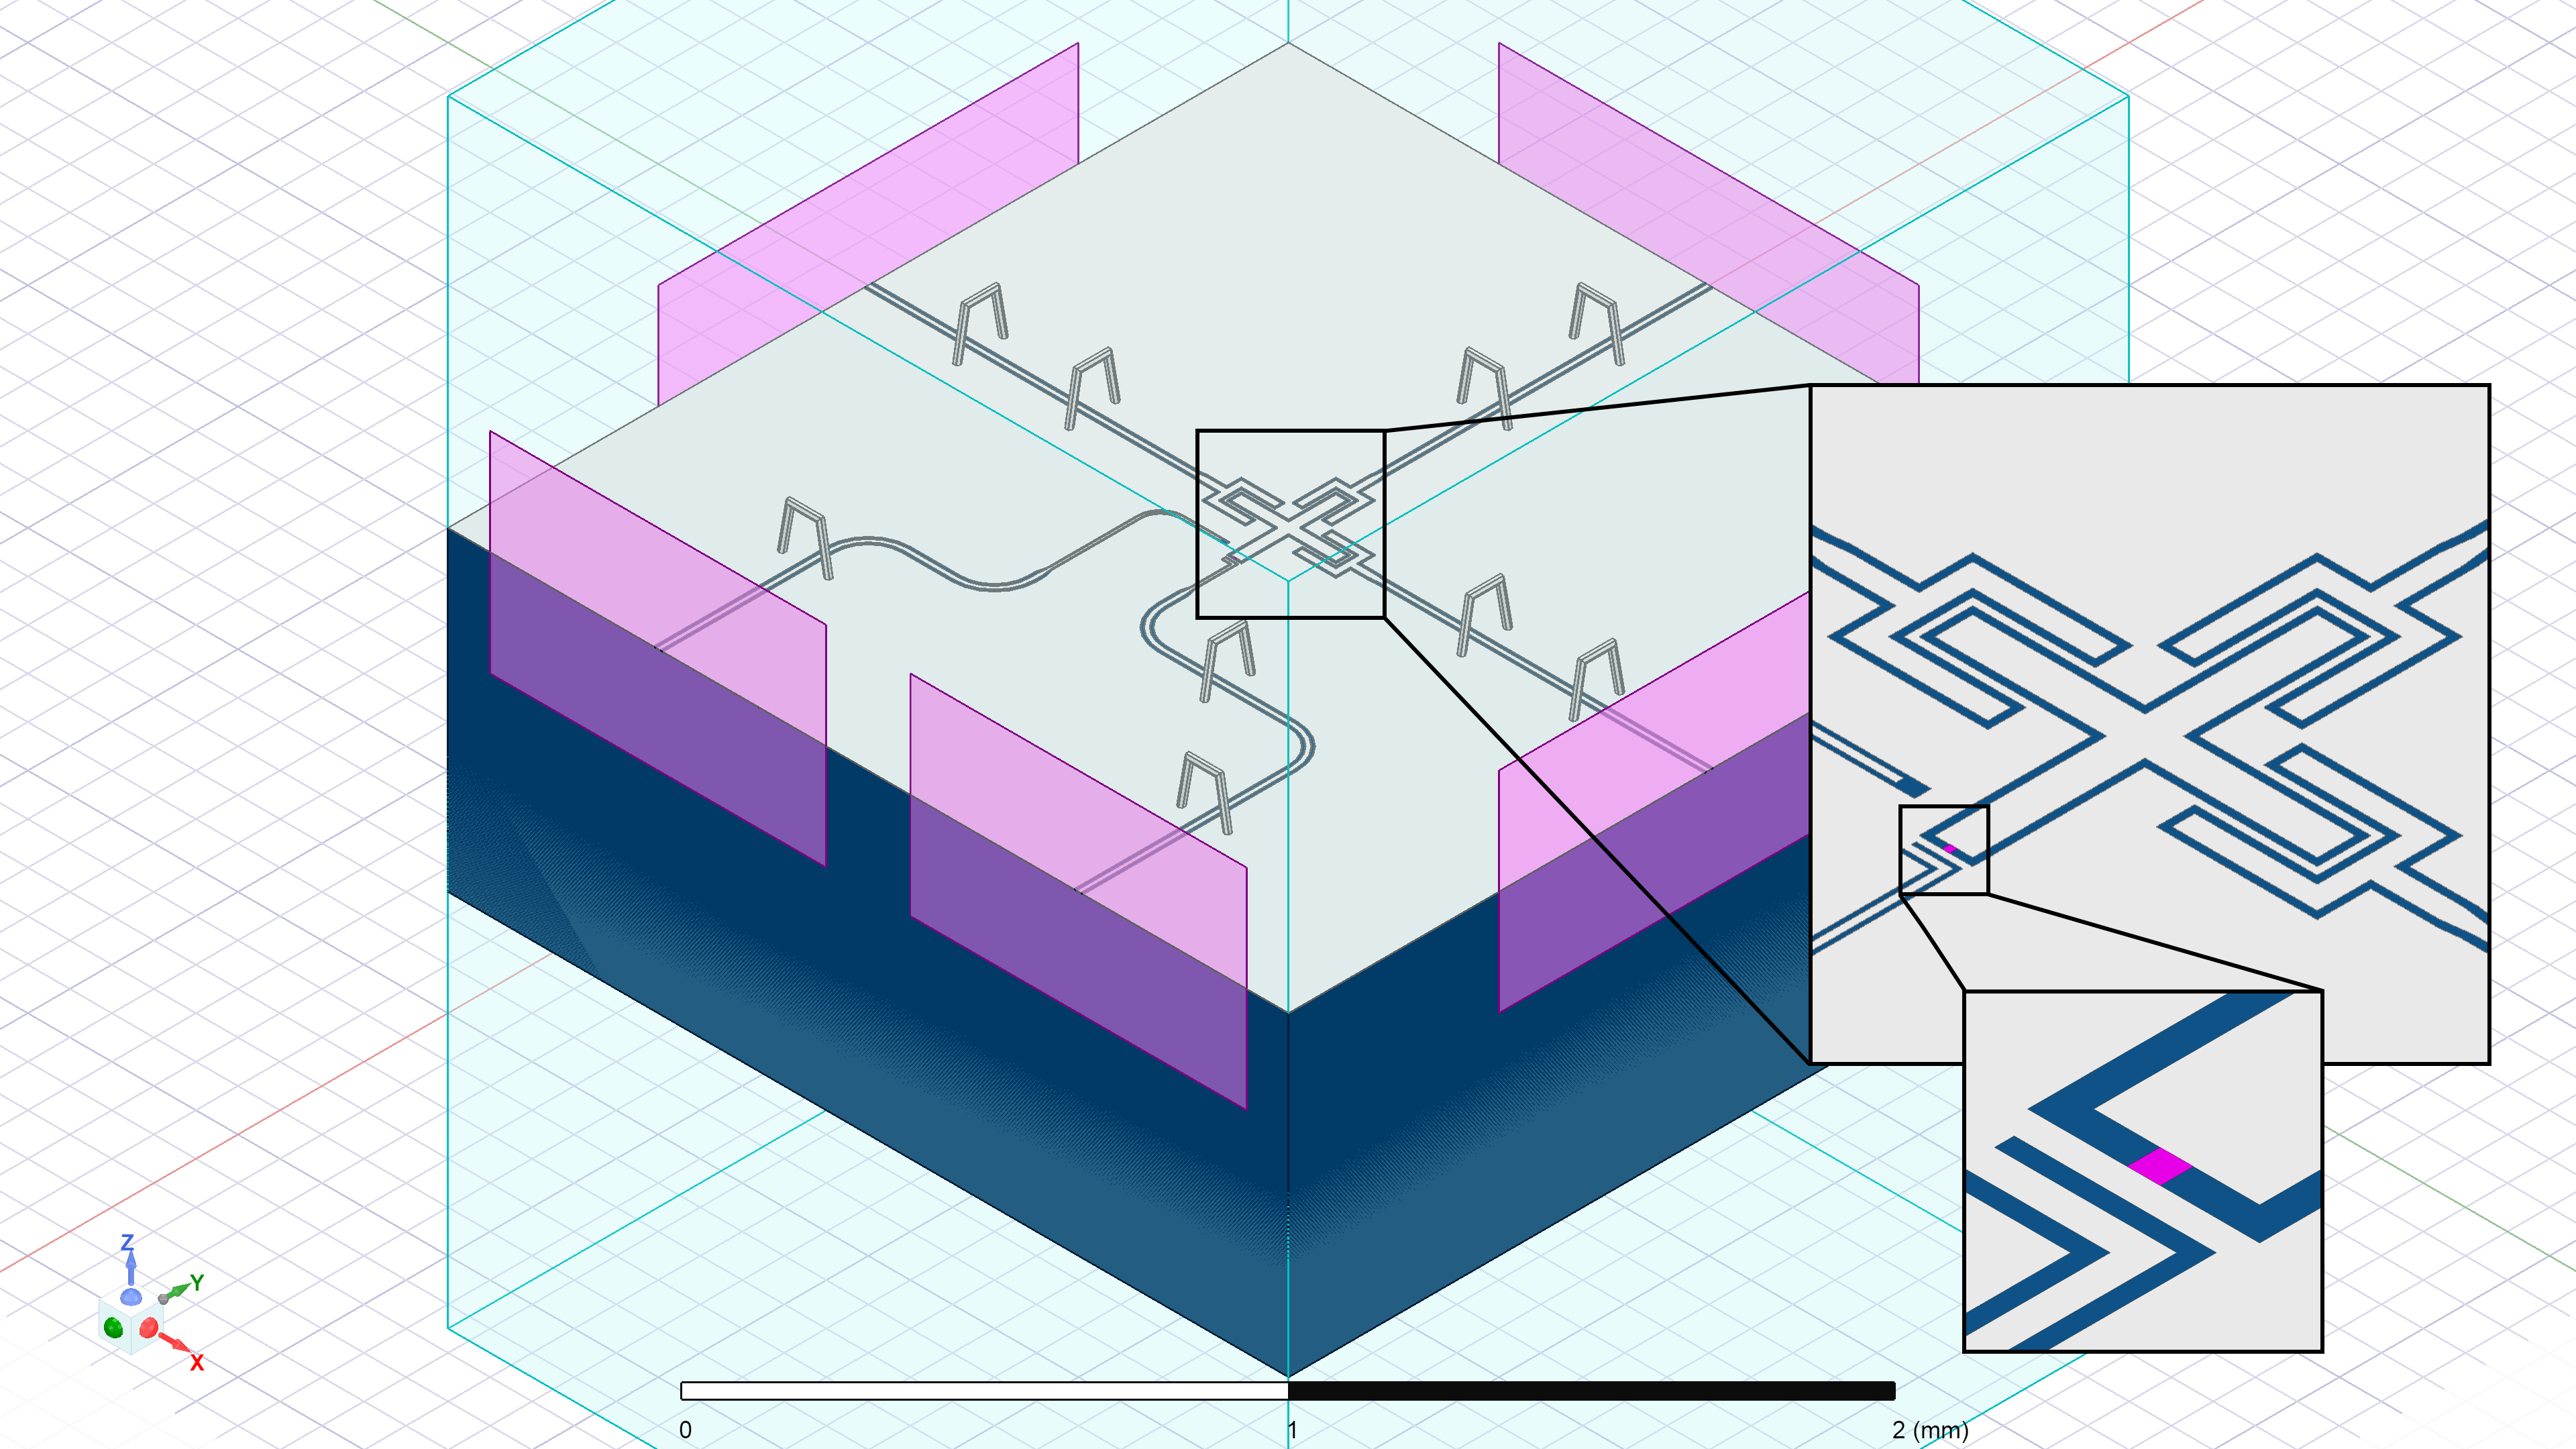
\includegraphics[width=\textwidth]{figures/xmon_extra_zoom.png}
    \caption{Brick model containing an Xmon style qubit \cite{xmon}. On the lower side of the cross, a lumped port (purple) is in the position where the SQUID would be located. Of the five wave ports on the boundary of the model, four correspond to CPW lines that are capacitively coupled to the qubit. The fifth wave port corresponds to a flux control line.}
    \label{fig:xmon_brick}
\end{figure}

Next, we look at a brick simulation that contains a transmon qubit. For qubits, we will have a lumped port that is located inside the boundaries of the simulation, unlike the wave ports previously seen. This lumped port is precisely the Josephson junction or ``qubit'' port that has been discussed in previous sections. The specific model we will discuss now is shown in Fig.\ \ref{fig:xmon_brick}. We want to use this model to discuss some more details that must be considered during the fitting process. When it comes to fitting this model, we need to be careful when dealing with the flux line port. Because the flux line is galvanically connected to the ground plane, it can be difficult to obtain a rational approximation of the form \ref{eq:impedance} with a positive definite DC residue. This is because the flux port components of the DC residue would be zero for a network like this. The fitting process can get close by including very small residue components and high frequency resonant modes, but this can cause unwanted effects in the Hamiltonian. To avoid these issues, we can fit the simulated impedance when the flux port is left open, and use this result when interconnecting with other bricks and constructing a Hamiltonian. However, we can still use the fit that includes the flux port for decay rate estimation. The results for fitting the simulated impedance for the model in Fig.\ \ref{fig:xmon_brick} are shown in Fig.\ \ref{fig:xmon_fit}. The fit including the flux line port struggles at low frequency due to the difficulty of attempting to fit the small residues and it also requires a number of poles outside of the visible frequency range. We would like to avoid including these types of poles when possible. When the flux port is left open, the fit for the remaining ports only requires one degenerate pole far out in the frequency range. We have found that allowing for a single degenerate pole when working with the electromagnetic models is sometimes needed for the fits to be accurate and this does not cause problems with the Hamiltonians. Sometimes, these degenerate poles and their residues can be thought of as an approximation to the infinite frequency pole that we have left out of (\ref{eq:impedance}).
\begin{figure}[!t]
    \centering
    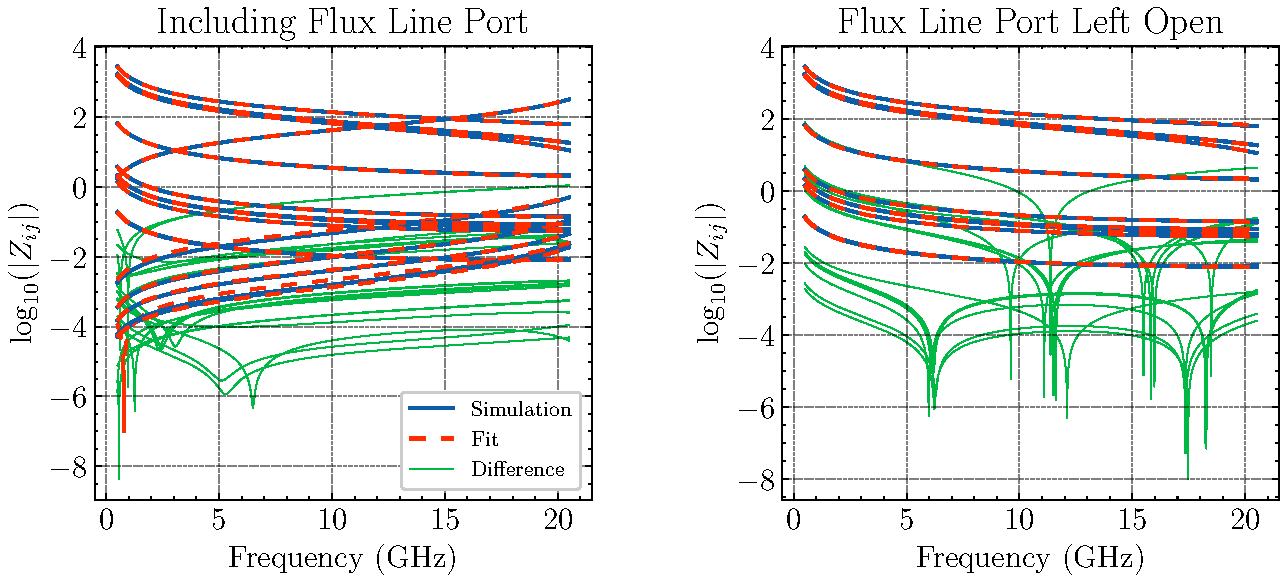
\includegraphics[width=\textwidth]{figures/xmon_fit.pdf}
    \caption{Impedance fit results for the simulation of the model shown in Fig.\ \ref{fig:xmon_brick}. On the left, the impedance including the flux line port is fitted. Note that the curves going to zero at low frequency on the left correspond to the parameters involving the flux line. In the fit on the right, the flux line port is left open to avoid inaccuracies brought in by trying to fit for the small residues corresponding to the flux line. All impedance parameters and differences between the fit and simulation are plotted together.}
    \label{fig:xmon_fit}
\end{figure}

When leaving the flux port open, we can obtain the Maxwell capacitance matrix that corresponds to the ports by inverting the DC residue. We then compare this to a Maxwell capacitance matrix obtained from a simulation in Ansys Q3D \cite{ansys_q3d}. In the Q3D simulation, the capacitance is computed between the metallic islands corresponding to the cross forming the Xmon and the CPWs leading to the boundary of the model. These matrices and differences are given in Appendix \ref{appendix:q3d_vs_hfss}. The differences are largest for the coupling capacitances that are small ($<$ 1 fF). Otherwise, estimates of the capacitance from fitting the HFSS model don't differ by more than 7\%. This difference is not caused by the fitting, and additional HFSS simulations and fits restricted to a low frequency range of 100 MHz to 1 GHz yield similar results. The differences likely come from the fact that the two simulation methods are different (HFSS is full-wave and Q3D is quasi-static) in addition to the different meshes and different port definitions in both models. There is the possibility to use Q3D within the HFSS simulation to solve the DC point, but with the combination of wave and lumped ports used in our models, this option is not available. For our examples here, we will use the models from HFSS, but it should be noted that improvements for the estimation at the DC point should be explored in the future within Ansys and potentially other simulation software.

\newpage

Taking a collection of bricks and their corresponding rational impedance functions, we can interconnect them to make a larger model. As an example, we consider the model in Fig.\ \ref{fig:triple_xmon}. In this model there are three resonator-coupled Xmon qubits. Each Xmon is also coupled to its own readout resonator that is also coupled to a common readout line. By looking at the S-parameters for this network, we clearly see which resonant modes couple the qubits to each other and to the feedline. Some of the relevant S-parameters are shown in Fig.\ \ref{fig:triple_xmon_S}.

\begin{figure}[h!]
    \centering
    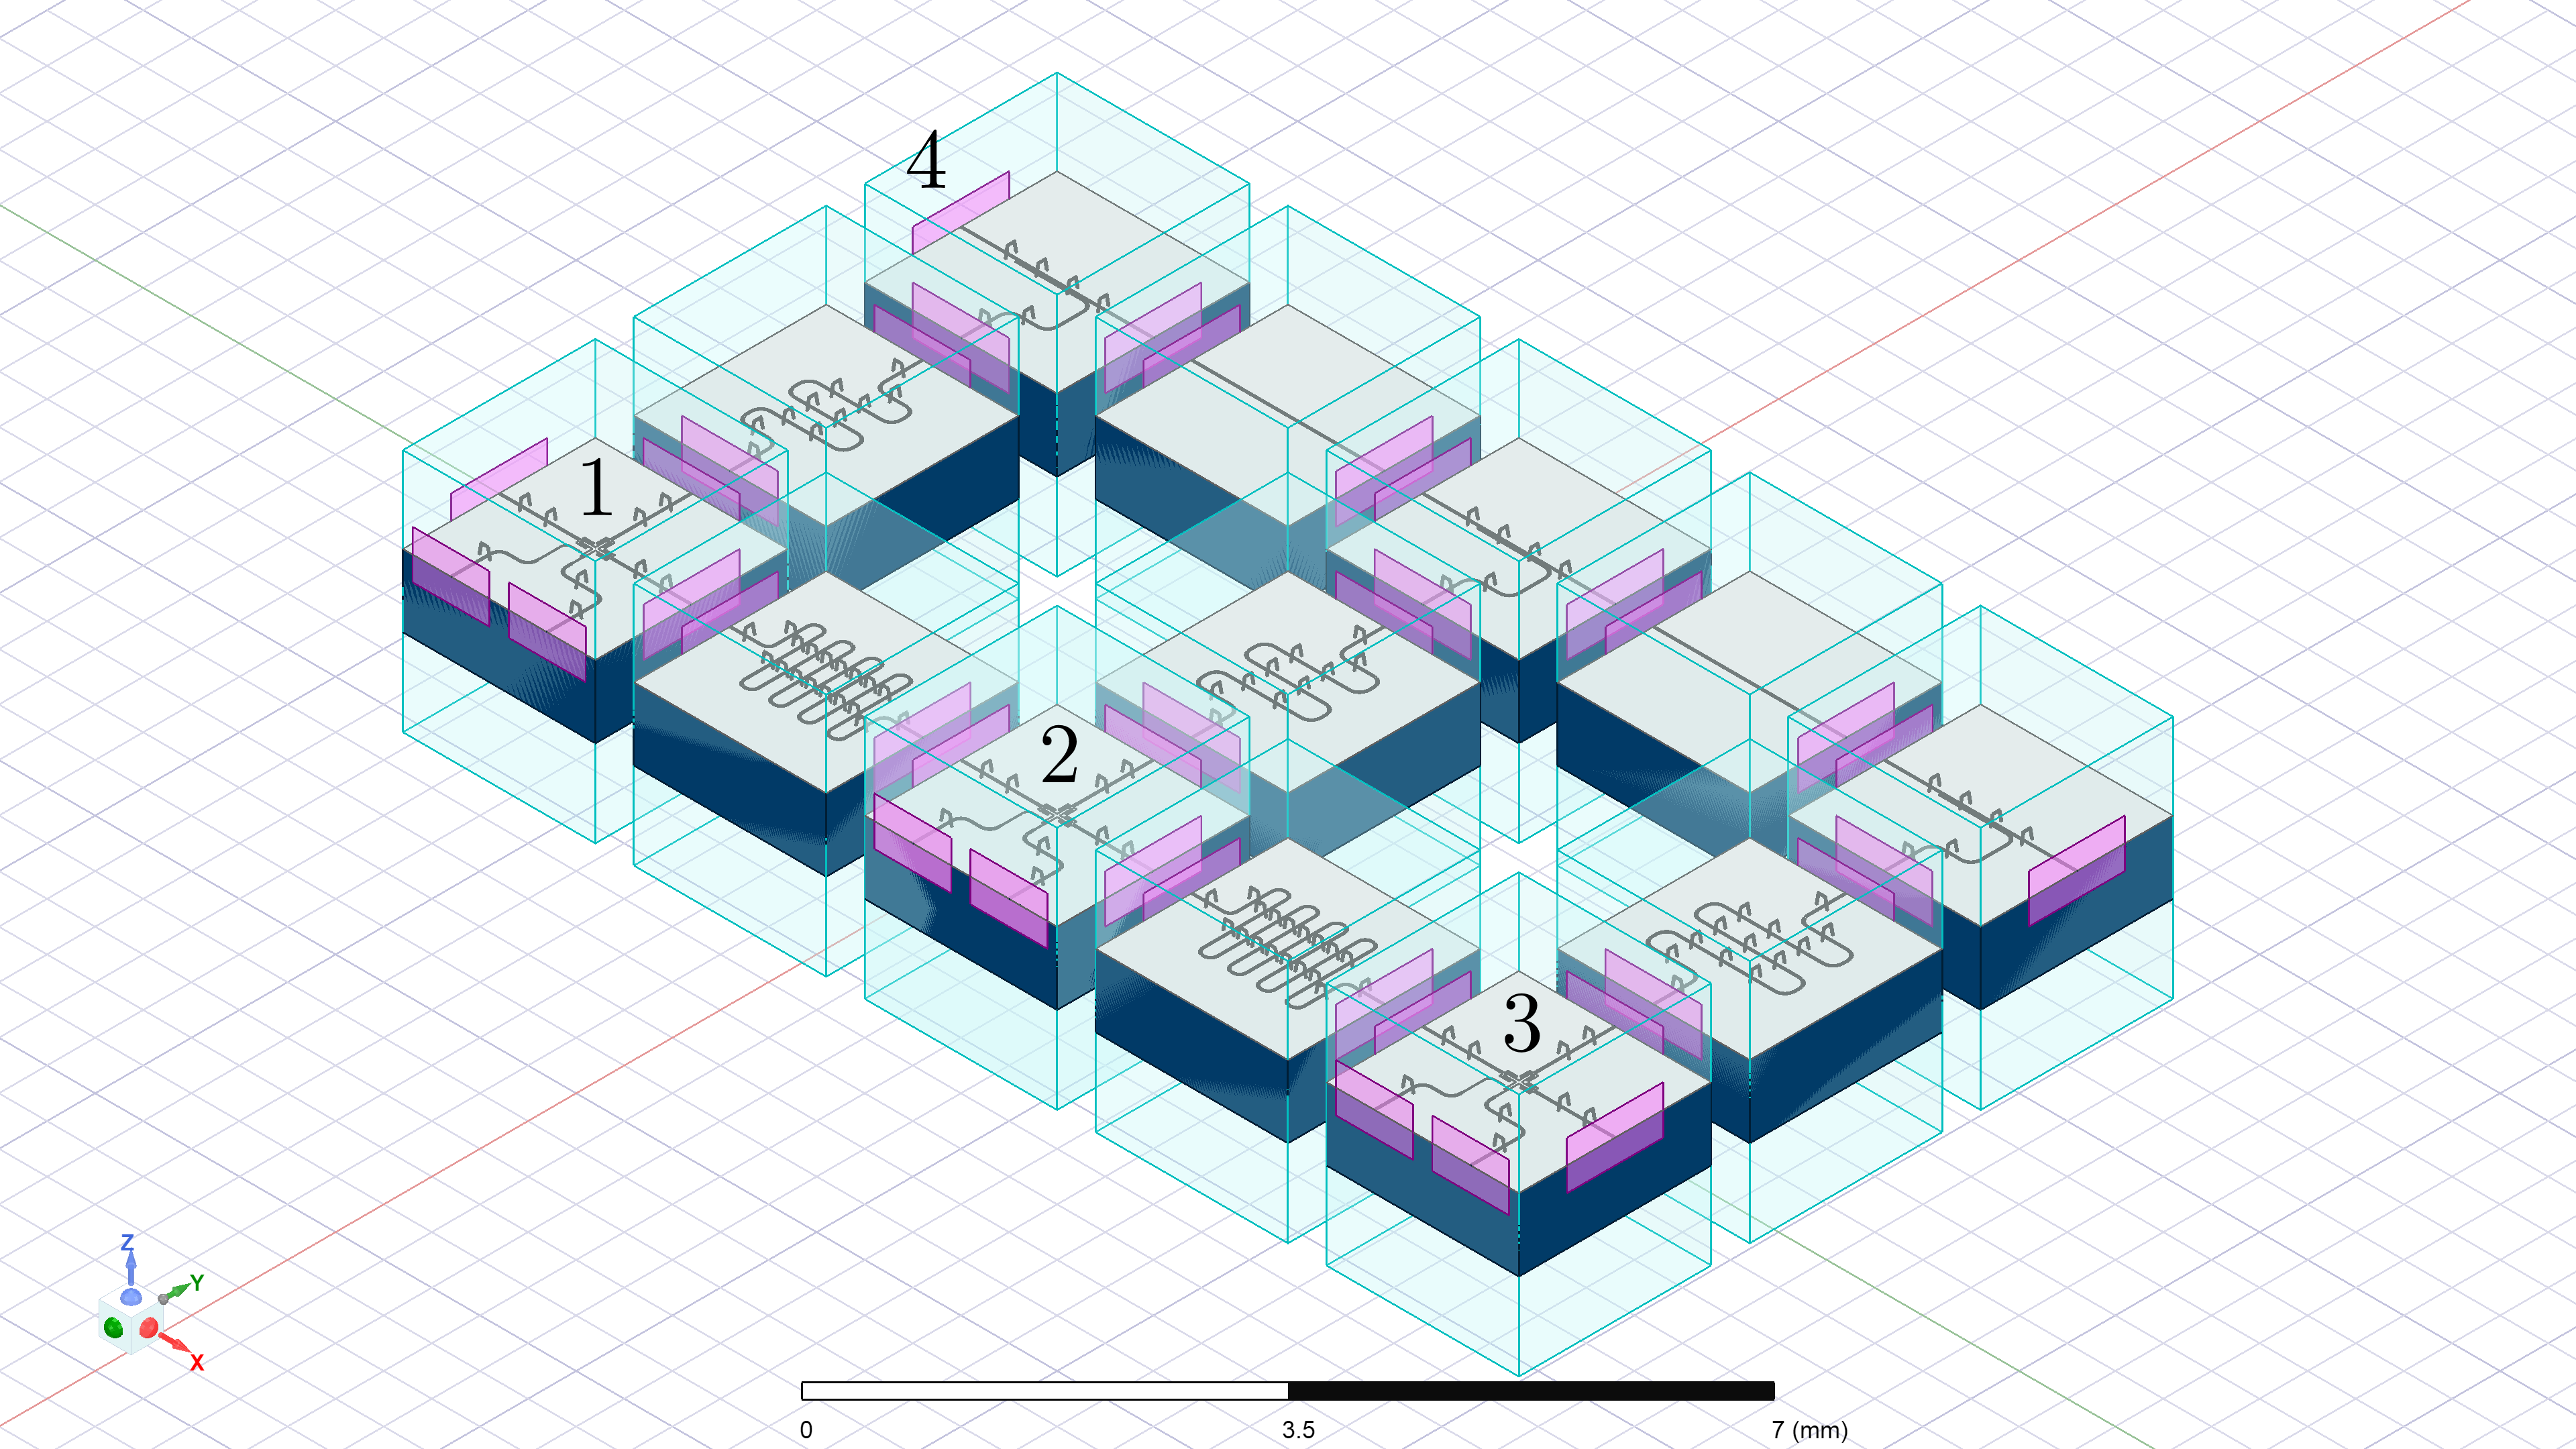
\includegraphics[width=\textwidth]{figures/triple_qubit_labeled.png}
    \caption{Brick model of a three Xmon circuit. The qubits are coupled to each other through half-wave resonators. Each qubit is also capacitively coupled to its own half-wave readout resonator that is capacitively coupled to a common readout line.}
    \label{fig:triple_xmon}
\end{figure}

\begin{figure}[h!]
    \centering
    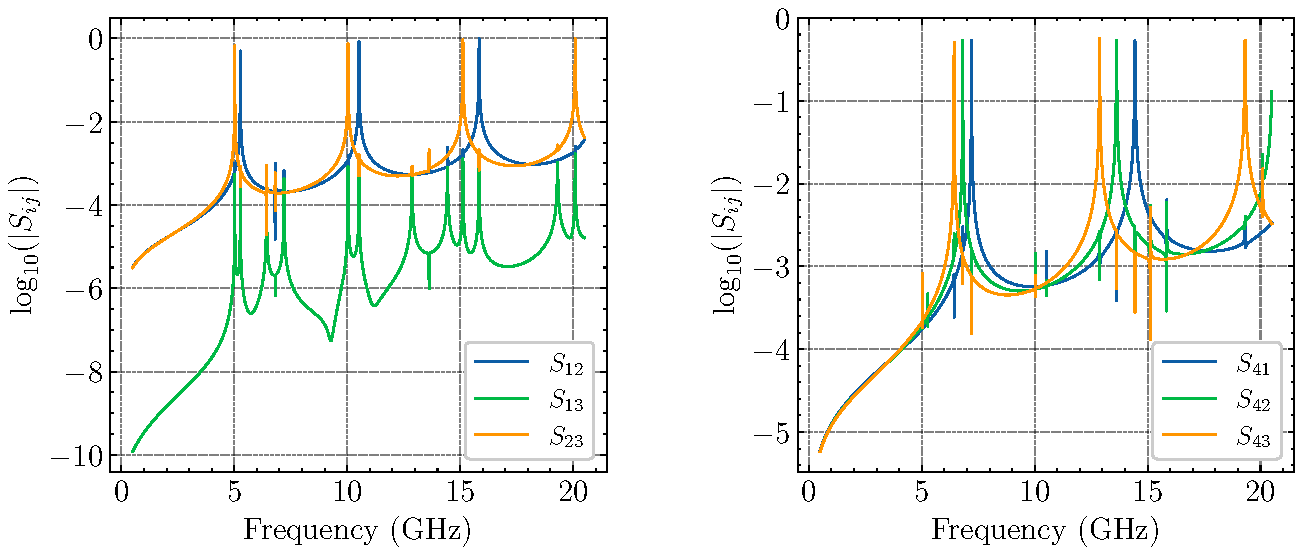
\includegraphics[width=\textwidth]{figures/three_qubit_S.pdf}
    \caption{Some of the matrix elements of the S-parameter for the fully interconnected network shown in Fig.\ \ref{fig:triple_xmon}. Port numbers are shown in Fig.\ \ref{fig:triple_xmon}. Ports 1-3 correspond to the three qubit junction ports. Port 4 corresponds to the left port of the feedline in Fig.\ \ref{fig:triple_xmon}.}
    \label{fig:triple_xmon_S}
\end{figure}

\newpage

With the rational impedance function corresponding to the fully interconnected model in Fig.\ \ref{fig:triple_xmon}, we can also build a circuit Hamiltonian of the form (\ref{eq:transmon_resonator_ham}). This can then be used to estimate the effective coupling rates between the qubits using (\ref{eq:eff_qubit_coupling}). We can also estimate the dispersive shift in the fundamental resonance frequency of each readout resonator using (\ref{eq:dispersive_shifts}). For the circuit in Fig.\ \ref{fig:triple_xmon}, these effective coupling rates and dispersive shifts are shown in Fig.\ \ref{fig:triple_xmon_geff_chi}. Additionally, with the fully interconnected model, we can estimate the relaxation times for each qubit by using (\ref{eq:matrix_eoms}) or (\ref{eq:qubit_decay_admittance}). The results for our example circuit in Fig.\ \ref{fig:triple_xmon} are shown in Fig.\ \ref{fig:triple_xmon_T1}.

\begin{figure}[h!]
    \centering
    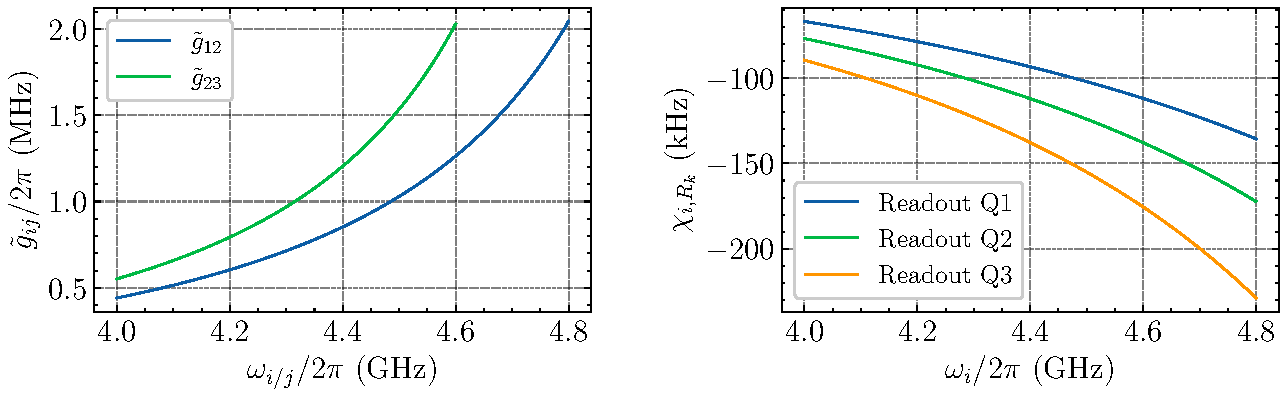
\includegraphics[width=\textwidth]{figures/three_qubit_geff_chi.pdf}
    \caption{Effective qubit coupling rates and readout resonator dispersive shifts for the interconnected model of Fig.\ \ref{fig:triple_xmon}. Left: Effective coupling rates between the qubits (third qubit is fixed at 4 GHz while the other two qubit frequencies are varied). The fundamental frequencies for the coupling resonators are 5.268 GHz ($Q1 \leftrightarrow Q2$) and 5.023 GHz ($Q2 \leftrightarrow Q3$). A cutoff frequency of 21.5 GHz is used for this example to avoid incorrect predictions of resonant modes outside the fitting range. Right: The dispersive shift in the fundamental modes of the readout resonators. The fundamental frequencies of the readout resonators for qubits 1 to 3 are 7.205 GHz, 6.812 GHz, and 6.435 GHz, respectively.}
    \label{fig:triple_xmon_geff_chi}
\end{figure}

\begin{figure}[h!]
    \centering
    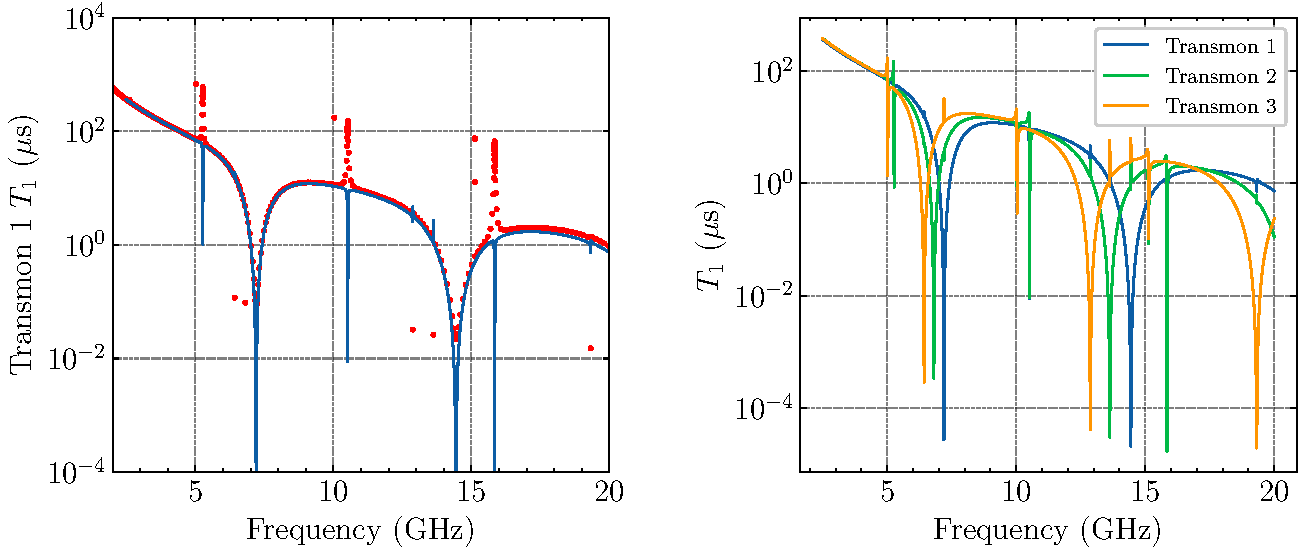
\includegraphics[width=\textwidth]{figures/three_qubit_T1.pdf}
    \caption{Relaxation times for the qubits in the circuit of Fig.\ \ref{fig:triple_xmon}. On the left plot, we focus only on qubit 1. For a sweep of the shunt inductance of qubit 1, the complex frequencies from (\ref{eq:matrix_eoms}) are plotted as red points. Isolated red points belong to the resonant modes that have a nearly fixed decay rate due to their small coupling to qubit 1. The blue line is the result of using (\ref{eq:qubit_decay_admittance}) with resistors shunting the external ports and no inductances shunting the qubit ports. On the right, we see the result from (\ref{eq:qubit_decay_admittance}) for all three qubits in the circuit.}
    \label{fig:triple_xmon_T1}
\end{figure}

Using these brick models, we can also estimate how the effective coupling through resonant modes present in a circuit will scale for multi-qubit devices. To do this, we recreate a qubit grid circuit similar to an example from \cite{solgun_sirf} where lumped elements were used. In our case, we use various bricks that correspond to electromagnetic models to create a grid of qubits. The circuit we consider is shown in Fig.\ \ref{fig:2x6}.

\begin{figure}[h!]
    \centering
    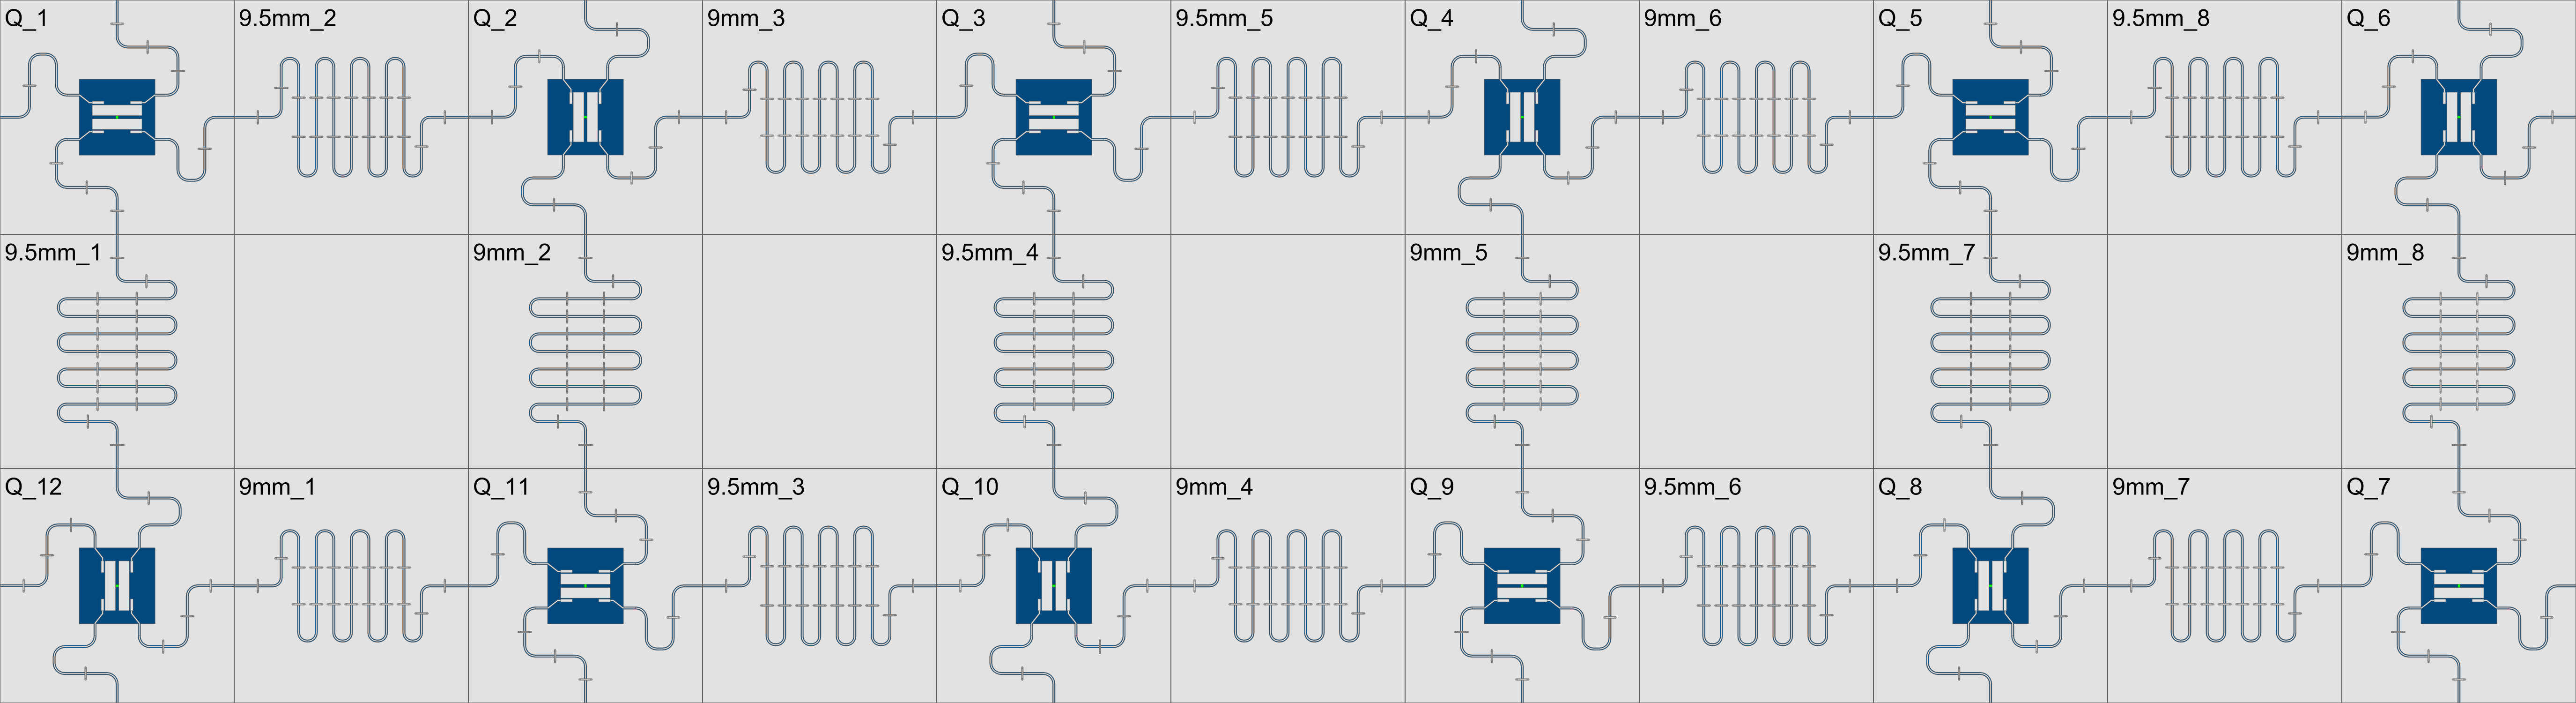
\includegraphics[width=\textwidth]{figures/2x6.png}
    \caption{A grid of IBM style transmons \cite{solgun_sirf} that are coupled through bus resonators. The qubits are numbered 1 to 12 starting from the top left and moving clockwise around the lattice.}
    \label{fig:2x6}
\end{figure}

After building the model of the circuit in Fig.\ \ref{fig:2x6}, we can compute the effective coupling rates between the qubits using (\ref{eq:eff_qubit_coupling}). The effective coupling of qubit 1 to all of the other qubits is shown in Fig.\ \ref{fig:2x6_coupling}. In this figure, we can see the exponential decay of the effective coupling as we get further from qubit 1. This exponential decay was also found for networks of this type in the lumped element example of \cite{solgun_sirf}. It is also expected for networks of this form if the direct capacitive coupling is excluded (see Appendix \ref{appendix:banded_cap}).

\begin{figure}[h!]
    \centering
    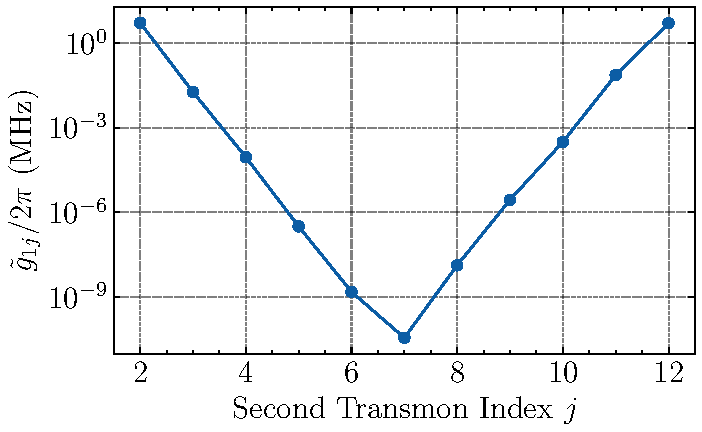
\includegraphics[width=0.5\textwidth]{figures/2x6_coupling.pdf}
    \caption{Effective coupling of qubit 1 of the circuit in Fig.\ \ref{fig:2x6} to all of the other qubits. All qubits are frequencies are fixed at 4.25 GHz. In practice, we would not see the influence of such small coupling rates $g/2\pi \lesssim 1$ kHz, but this can still be a useful tool for verifying that the long range coupling through resonant modes in a specific layout is negligible.}
    \label{fig:2x6_coupling}
\end{figure}

\subsection{Parasitic Resonances}
As the number of components present within superconducting circuits increases, we may start to see parasitic resonances at frequencies closer to the operating frequency range of the qubits. These parasitic resonances at lower frequencies could have a non-negligible impact on the effective coupling between qubits. Depending on where these resonant modes arise (physically and in frequency), it is be useful to see how changes to device geometry results in changes of the couplings to these parasitic resonances.

As an example, we consider a parasitic resonance that is present within a chain of Xmons. The parasitic resonance we will be concerned with is the lowest resonant mode of the chain structure that is above the operating frequencies of the qubits (around 4 to 6 GHz). Of course, there will be higher frequency parasitic resonances, but here we only consider the lowest as it should be the mode that contributes the most to any changes in effective coupling. In Fig.\ \ref{fig:xmon_1x3_eig}, we can see the electric field profile of the lowest resonant mode in a chain of three Xmons. The field profile and resonance frequency are found using the eigenmode solver within HFSS. While not super clear with just three Xmons, the outer two crosses participate less in the resonance than the center cross. This is clearer if we increase the length of the chain as shown in Fig.\ \ref{fig:xmon_1x10_eig}. We can also see that when adding more Xmons to the chain, the frequency of the parasitic resonance in the chain decreases. Using the eigenmode solver in HFSS, we obtain the results in Fig.\ \ref{fig:xmon_chain_res} that show how the frequency of the resonance decreases as we increase the number of Xmons.
\begin{figure}[h!]
    \centering
    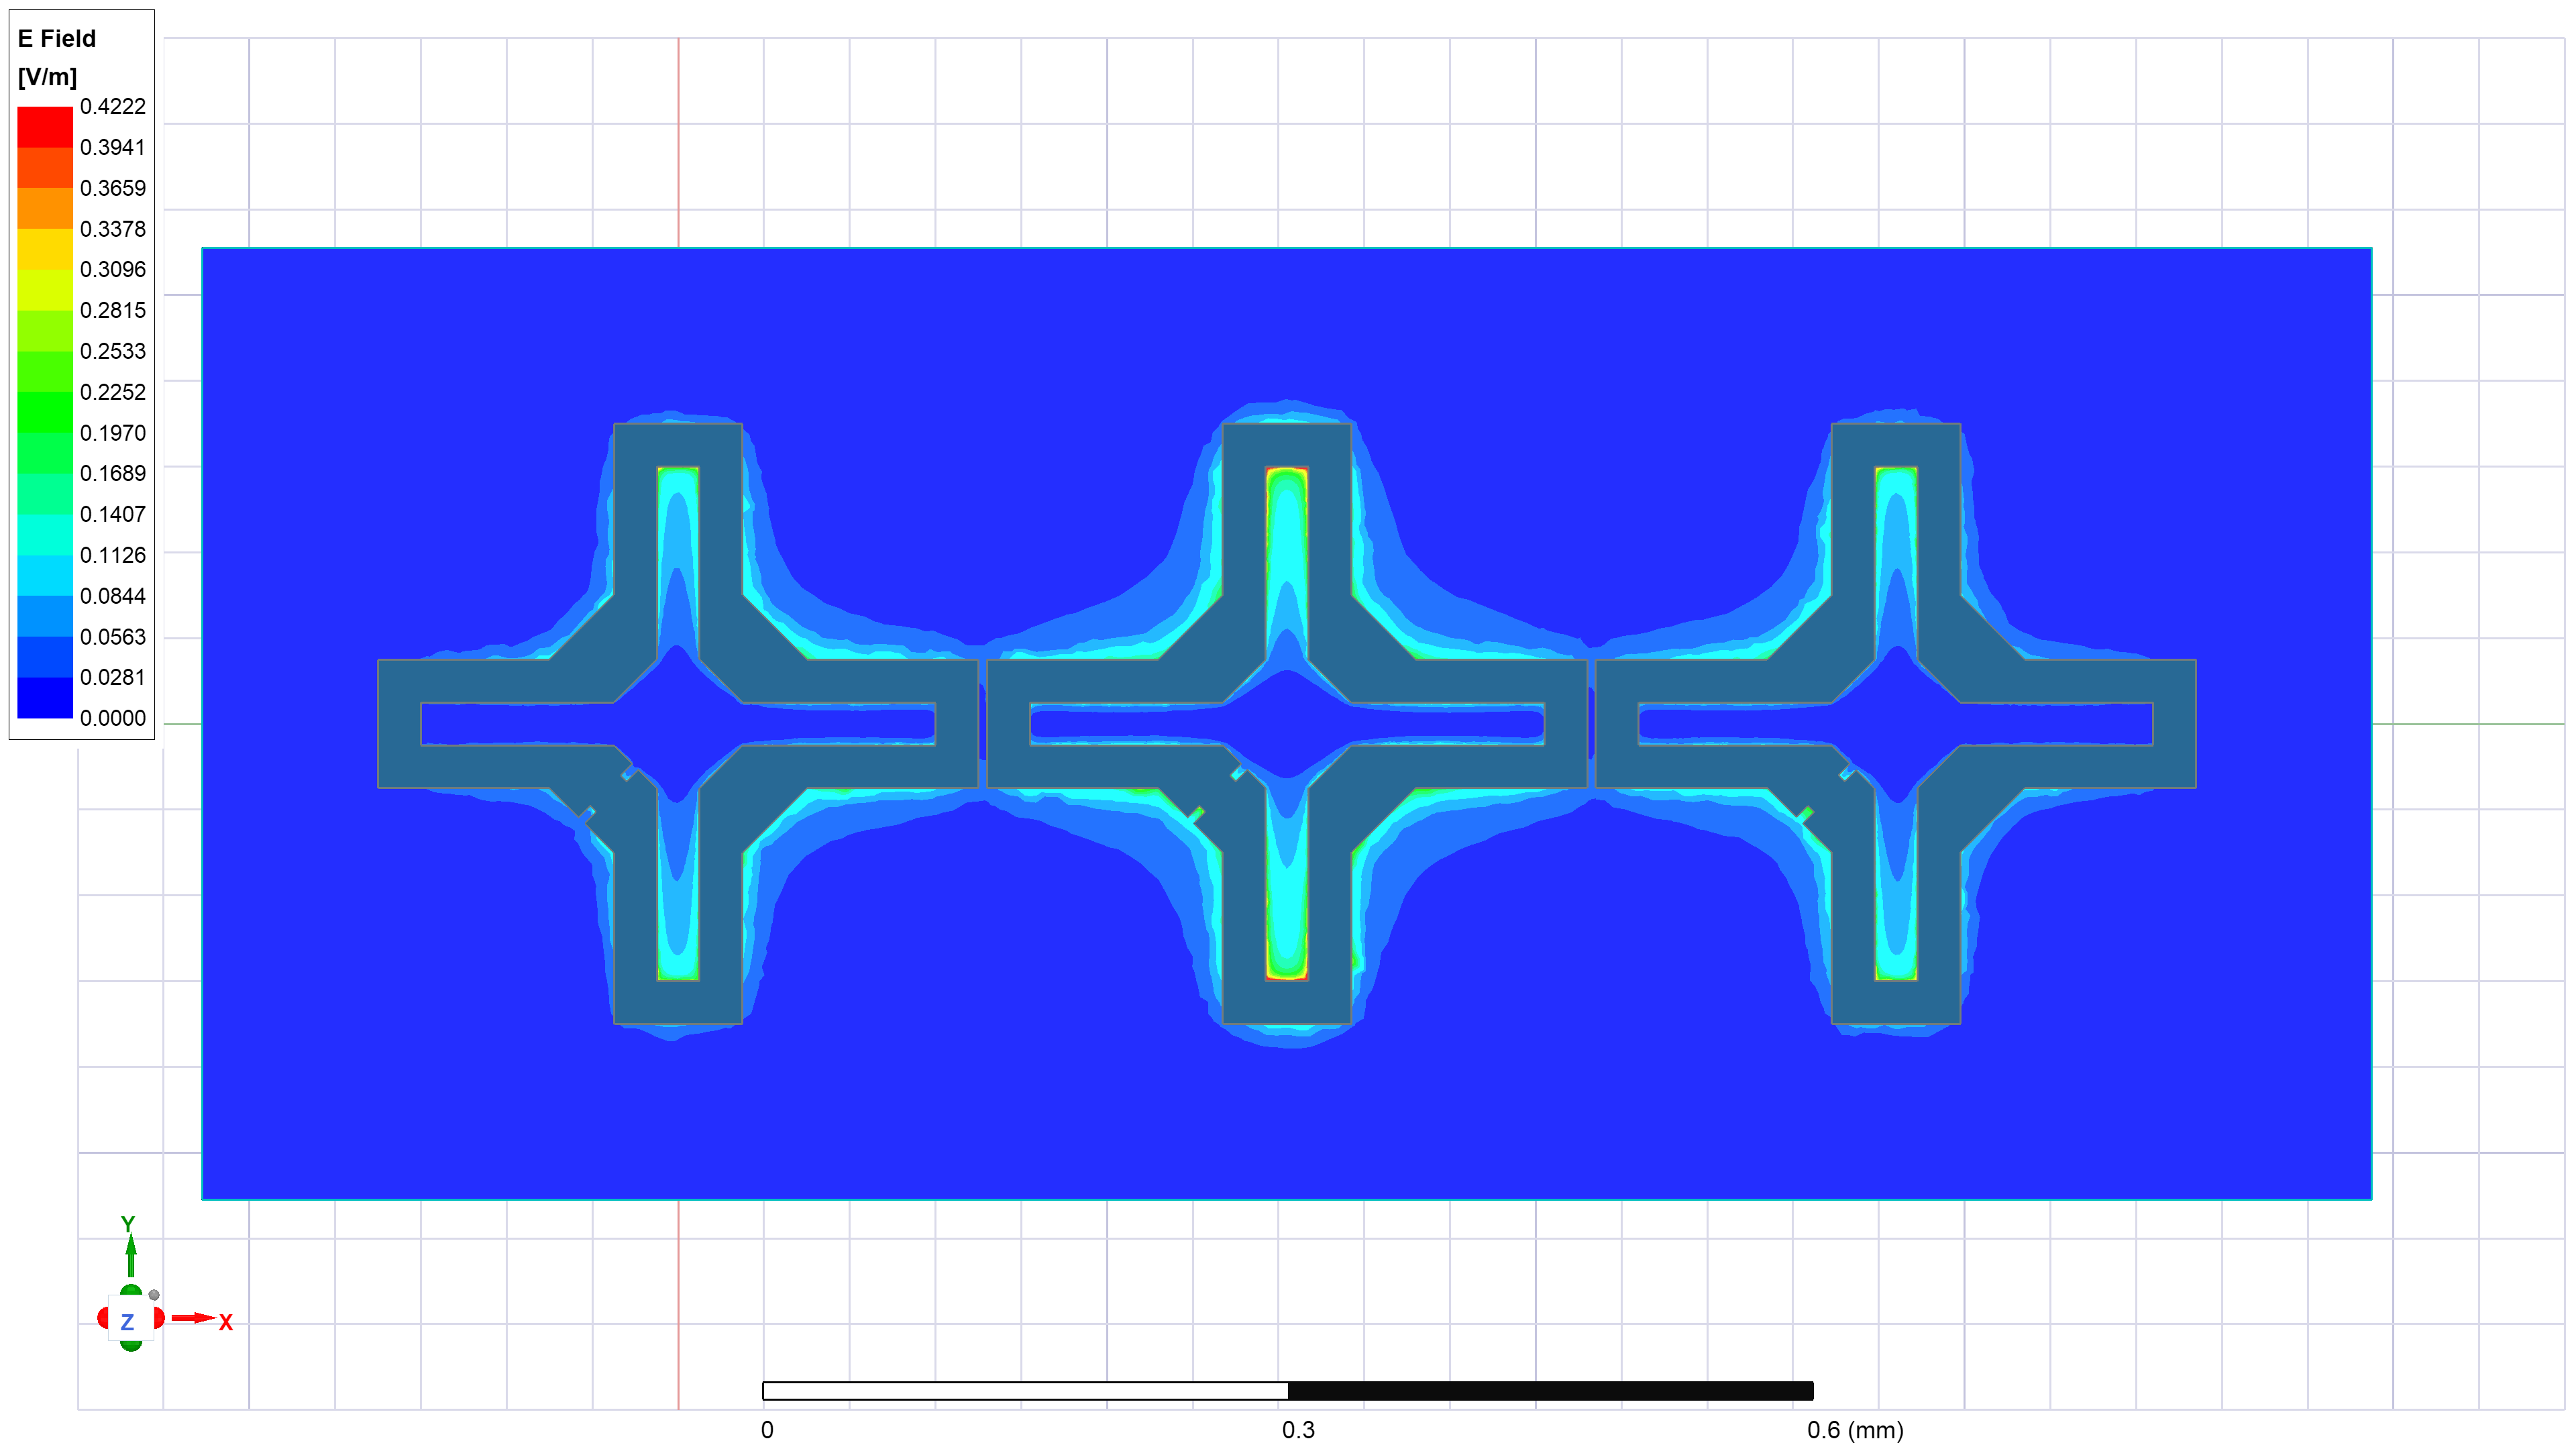
\includegraphics[width=0.75\textwidth]{figures/xmon_1x3_eig.png}
    \caption{Magnitude of the electric field at the surface of the perfect conductor in a three Xmon chain. This is the lowest resonant mode above the operating range of the qubits. The resonant frequency is 52.5322 GHz.}
    \label{fig:xmon_1x3_eig}
\end{figure}

\begin{figure}[h!]
    \centering
    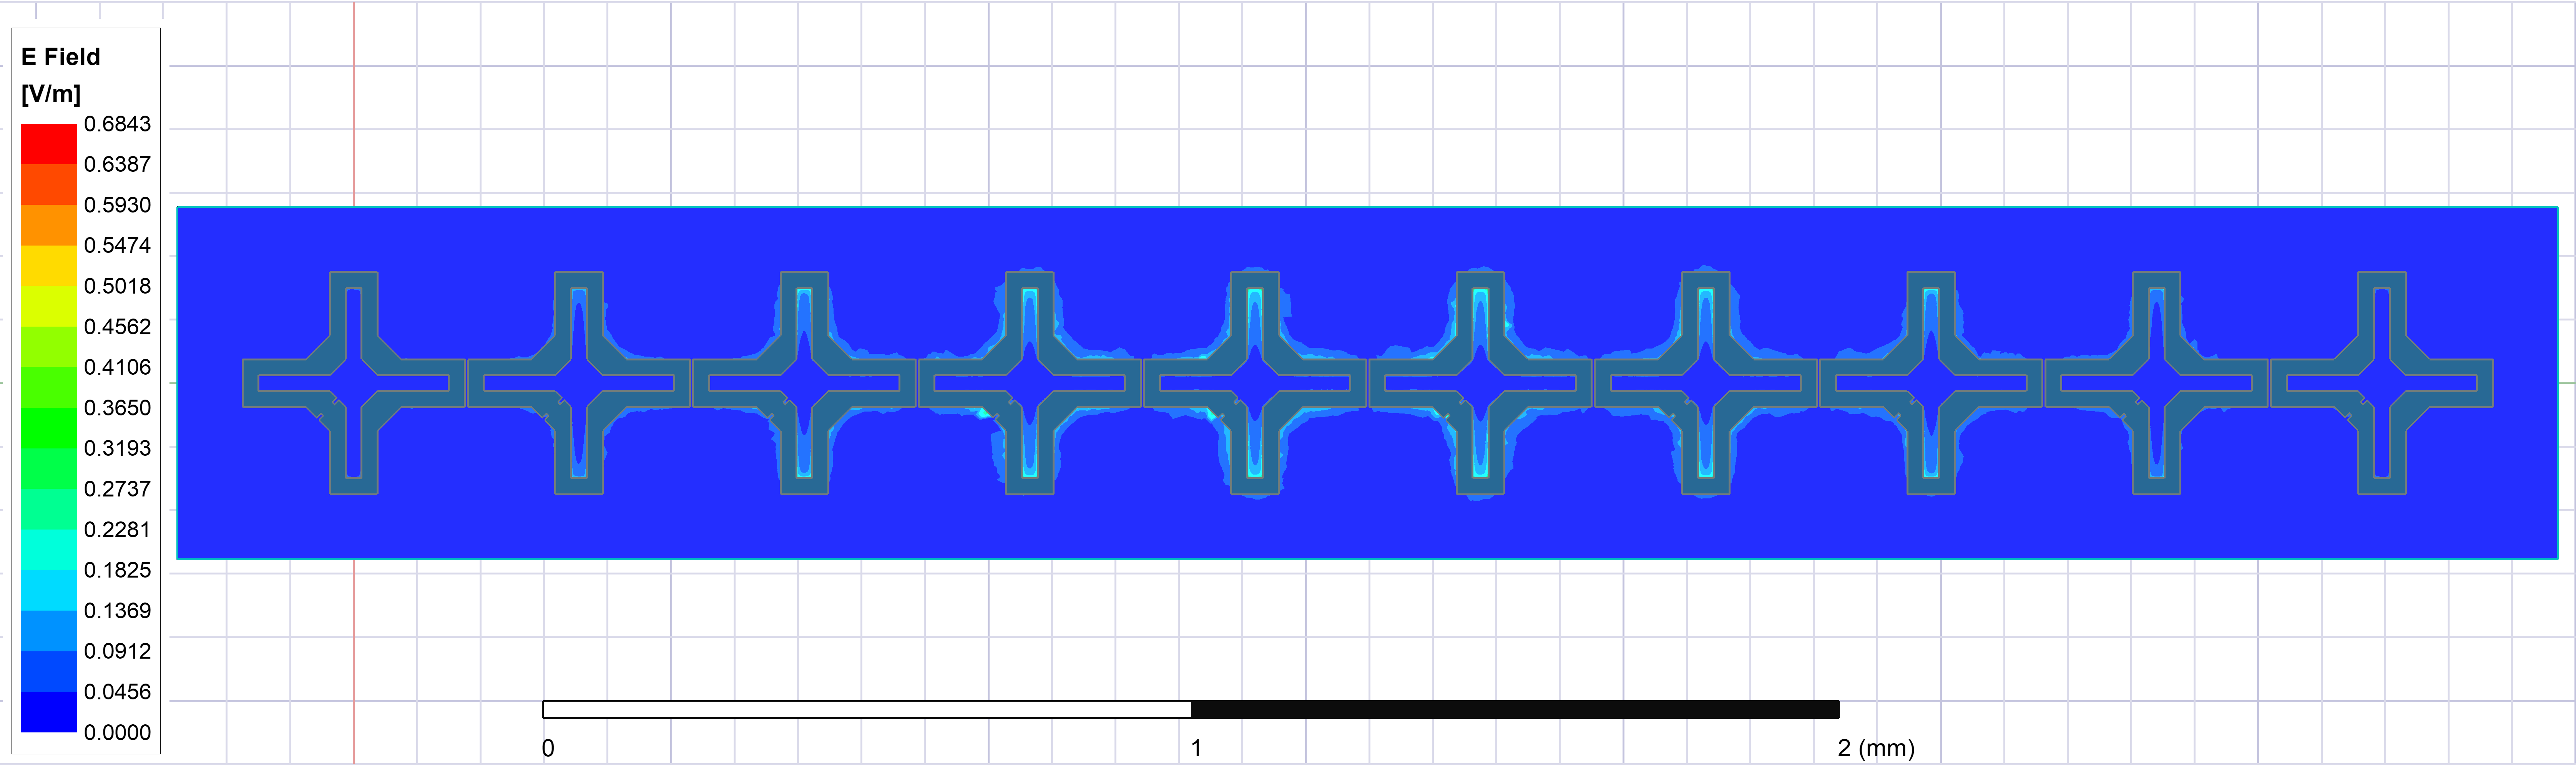
\includegraphics[width=\textwidth]{figures/xmon_1x10_eig.png}
    \caption{Magnitude of the electric field in a ten Xmon chain for the lowest resonant mode of 37.8159 GHz in the structure.}
    \label{fig:xmon_1x10_eig}
\end{figure}

To estimate the coupling rates of the qubits to this parasitic resonance, we can try to use the vector fitting methods of Section \ref{section:vector_fitting}. Including lumped ports at the positions of the junctions, we obtain the impedance parameter in HFSS over a broad frequency range (1 GHz to 80 GHz) so that the lower parasitic resonance is visible. Unfortunately, the traditional vector fitting struggles to give a good fit for the whole frequency range with the results shown in Fig.\ \ref{fig:xmon_3_4_fit}. Due to the poor fit, the estimated coupling rates are likely inaccurate. We can alternatively look at the S-parameters to understand how the qubits are coupled to the parasitic resonance relative to one another. This can also be used to track how coupling to parasitic resonances changes for different device geometry. In Fig.\ \ref{fig:xmon_3_4_S} we can see the diagonal matrix elements of the S-parameters for the three and four Xmon chains. This clearly shows which qubits are most strongly coupled to the parasitic resonance. If changes are made to the device, we can potentially track how the S-parameters compare between devices to see if the coupling of the qubits to these parasitic resonances has gone down. In Fig.\ \ref{fig:xmon_5_6_S} we show similar plots for the five and six Xmon chains.

\begin{figure}[h!]
    \centering
    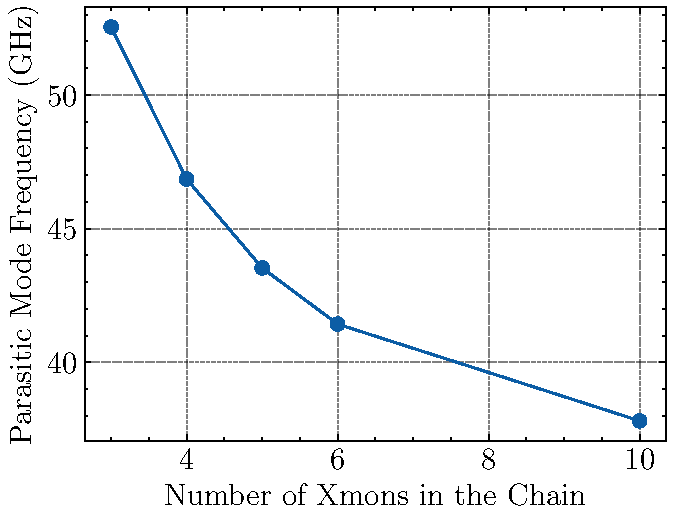
\includegraphics[width=0.5\textwidth]{figures/xmon_chain_res.pdf}
    \caption{Lowest parasitic resonance frequencies for different numbers of Xmons in a chain. Resonance frequencies are computed using the eigenmode solver within HFSS.}
    \label{fig:xmon_chain_res}
\end{figure}

\begin{figure}[h!]
    \centering
    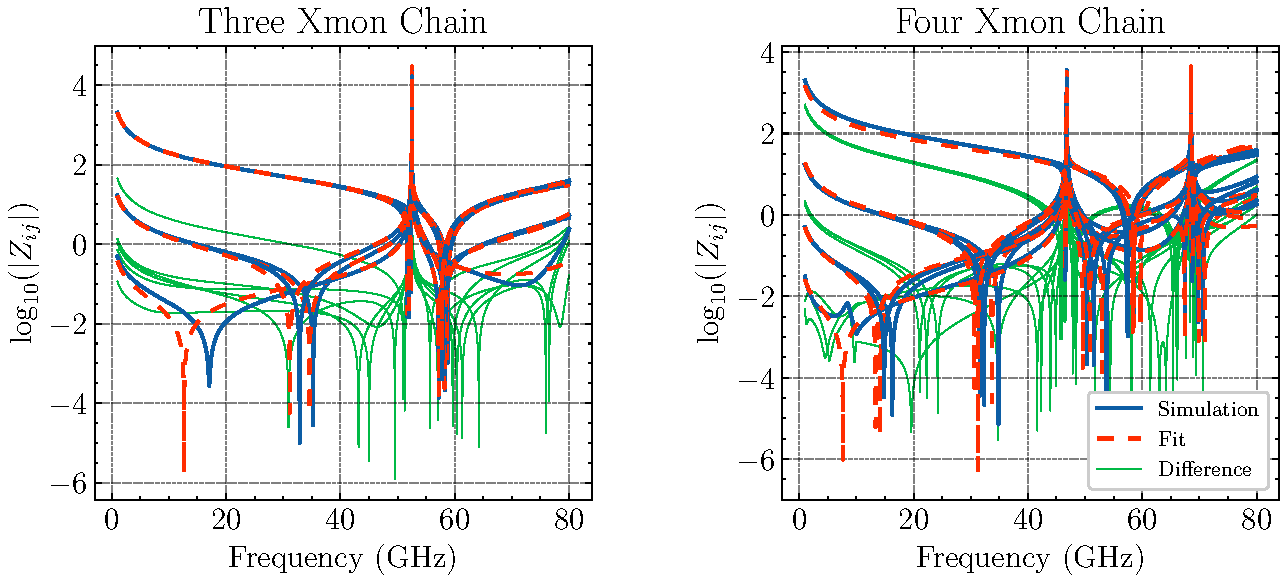
\includegraphics[width=\textwidth]{figures/xmon_chain_fitting.pdf}
    \caption{Attempts at fitting the impedance parameter for the three and four Xmon chains. For the three qubit chain shown in Fig.\ \ref{fig:xmon_1x3_eig}, we find that magnitudes of the coupling rates of the three qubits to the lowest parasitic resonance mode are 103, 228 and 167 MHz from left to right. For the four qubit chain, the magnitudes of the coupling rates are 129, 292, 321 and 204 MHz. This is for the qubit frequencies fixed at 4 GHz. The coupling rates are not symmetric due to the junction ports being off center on each cross. Due to the poor fitting of the DC and parasitic resonance residues, the coupling rates are likely inaccurate as we expect the coupling rates of the qubits to the resonance to be lower in the four Xmon chain (see Fig.\ \ref{fig:xmon_3_4_S}).}
    \label{fig:xmon_3_4_fit}
\end{figure}

\newpage

\begin{figure}[!ht]
    \centering
    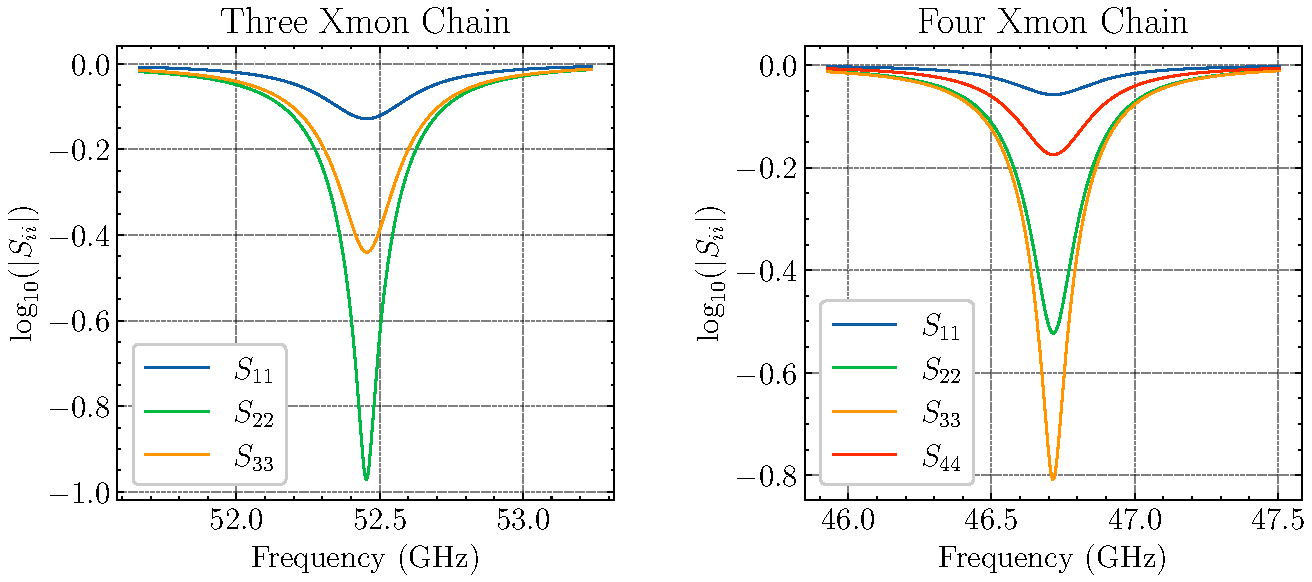
\includegraphics[width=\textwidth]{figures/xmon_chain_S.pdf}
    \caption{Diagonal matrix elements of the S-parameters for the three and four Xmon chains. The qubit ports are numbered left to right on the chain. We can see that closer to the center of the chain, the qubits are more strongly coupled to the parasitic resonance. Also, we can see that in the four Xmon chain, the qubits are coupled less to the parasitic resonance than in the three Xmon chain.}
    \label{fig:xmon_3_4_S}
\end{figure}

\begin{figure}[!ht]
    \centering
    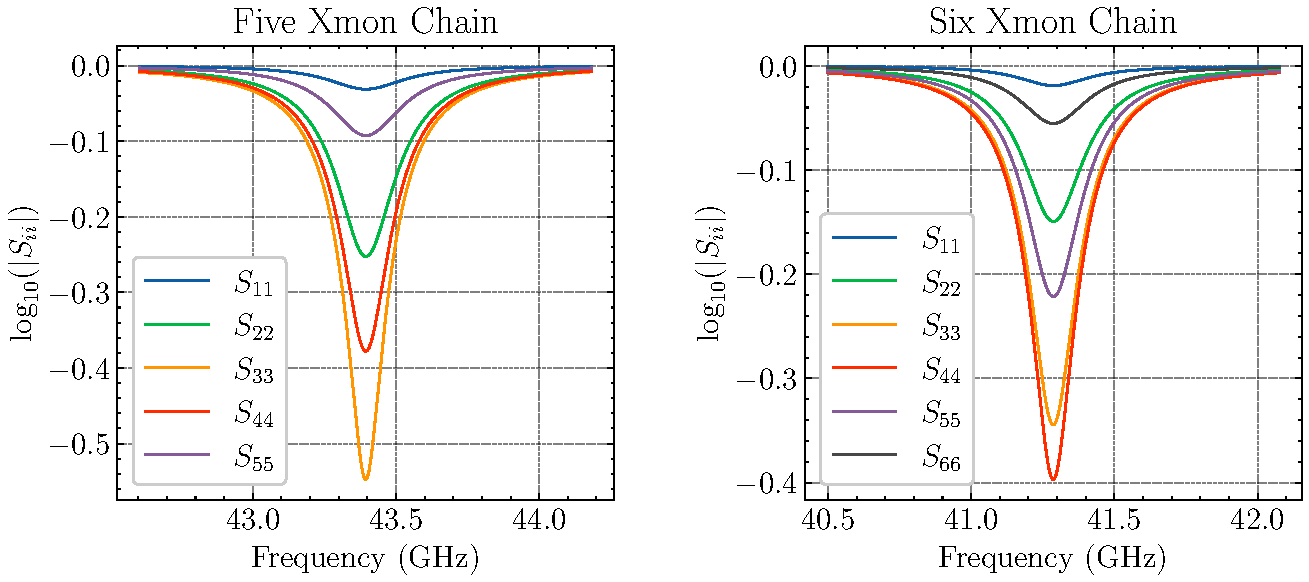
\includegraphics[width=\textwidth]{figures/xmon_chain_S_5_6.pdf}
    \caption{Similar to Fig.\ \ref{fig:xmon_3_4_S}, but for the five and six Xmon chains.}
    \label{fig:xmon_5_6_S}
\end{figure}
